\documentclass[review]{elsarticle}
%% Latex documents that need direct input
%  The subcaption package allows for subfloat figure within a single float.
%  This package substitutes the depregated subfigure and subfig packages 
%  allowing to have subfigures within figures, or subtables within table 
%  floats. Subfloats have their own caption, and an optional global 
%  caption. 
%  >> WARNING: some journal templates from Springer and IEETrans might not
%              be compatible with this package forcing to use the 
%              deprecated packages instead.
% \usepackage{subcaption}
% \usepackage{subfig}
\usepackage{subfigure}

%% color package
\usepackage[table]{xcolor}
\usepackage{color}

%% Colorpackage for table
\usepackage{colortbl}
\usepackage{tabularx}
\usepackage{arydshln}

%  The following command loads a graphics package to include images
%  in the document. It may be necessary to specify a DVI driver option,
%  e.g., [dvips], but that may be inappropriate for some LaTeX
%  installations.
\usepackage[]{graphicx}

% Document structure package
%
\usepackage{standalone}

%%% STOP USING FUCKING PACKAGE WHICH A FUCKING USELESS
% In order to include files without having a clear page using \include*,
% the newclude package is required
%\usepackage{newclude}

\usepackage{array}

% Required for acronyms
% use \acresetall to reset the acroyms counter
% macros=True, allows for calling \myTriger rather than \ac{myTriger}
\usepackage[single=true, macros=true, xspace=true]{acro}

%%%%%%%%%%%%%%%%%%%%%%%
%% Elsevier bibliography styles
%%%%%%%%%%%%%%%%%%%%%%%
%% To change the style, put a % in front of the second line of the current style and
%% remove the % from the second line of the style you would like to use.
%%%%%%%%%%%%%%%%%%%%%%%

%% Numbered
%\bibliographystyle{model1-num-names}

%% Numbered without titles
%\bibliographystyle{model1a-num-names}

%% Harvard
%\bibliographystyle{model2-names.bst}\biboptions{authoryear}

%% Vancouver numbered
%\usepackage{numcompress}\bibliographystyle{model3-num-names}

%% Vancouver name/year
%\usepackage{numcompress}\bibliographystyle{model4-names}\biboptions{authoryear}

%% APA style
%\bibliographystyle{model5-names}\biboptions{authoryear}

%% AMA style
%\usepackage{numcompress}\bibliographystyle{model6-num-names}

%% `Elsevier LaTeX' style
\bibliographystyle{elsarticle-num}
%%%%%%%%%%%%%%%%%%%%%%%



\usepackage{booktabs}
\usepackage{datatool}
\usepackage{multirow}
%\usepackage{arydshln}
%\usepackage{tabularx}
\usepackage{courier}
\usepackage{lscape}
\usepackage{pdflscape}


% packages for checkmark 
\usepackage{bbding}
\usepackage{pifont}
\usepackage{wasysym}
\usepackage{amssymb}

\newcommand{\cmark}{\large \color{green!60!black!80}\ding{51}}
\newcommand{\mmark}{\large {\color{green!60!black!80}\ding{51}}$^{!}$}
\newcommand{\xmark}{\large \color{red!60!black!80}\ding{55}}
\newcommand{\cmarksmall}{\color{green!60!black!80}\ding{51}}
\newcommand{\mmarksmall}{{\color{green!60!black!80}\ding{51}}$^{!}$}
\newcommand{\xmarksmall}{\color{red!60!black!80}\ding{55}}
% Clever cross referencing. Using cleverref, instead of writting
% figure~\ref{...} or equation~\ref{...}, only \cref{...} is required.
% The package interprates the references and introduces the figure, fig.,
% equation, eq., etc keywords. \Cref forces first letter capital.
% >> WARNING: This package needs to be loaded after hyperref, math packages,
%             etc. if used.
%             Cleveref is recomended to load late
% \usepackage{hyperref}
\usepackage{cleveref}

% SI units
\usepackage{siunitx}
% Define the money way to write
\sisetup{
  group-four-digits = true,
  group-separator = {,}
}
\DeclareSIUnit\px{px}

% Package for math symbol for vector
\usepackage{bm}
\usepackage[titletoc,toc,title]{appendix}

% Package tikz
\usepackage{scalefnt,tikz,xifthen}
\usetikzlibrary{fit, patterns, shapes, backgrounds, positioning}
\usetikzlibrary{shadows,arrows,calc,positioning,backgrounds,snakes,decorations.text,decorations.markings,shapes,patterns,fit,chains,decorations.pathreplacing}    % contains the latex packages
% See the number of line
\usepackage{lineno}
\modulolinenumbers[5]

% Managing TODOES and unfinished figures
\usepackage{todonotes}

% Some packages useful for edition
\usepackage{changebar}
\usepackage{changes}

% Change the top rule
\newcommand*\ctoprule[1]{\addlinespace\cmidrule[\heavyrulewidth]{#1}}  % packages to facilitate editing
%%%%%%%%%%%%%%%%%%%%%%%%%%%%%%%%%%%%%%%%%%%%%%%%%%%%%%%%%%%%% 
%>>>> uncomment following for page numbers
% \pagestyle{plain}    
%>>>> uncomment following to start page numbering at 301 
%\setcounter{page}{301} 
\definechangesauthor[name={sik}, color=blue]{sik}
\setremarkmarkup{(#2)}
        % contains package and variables init.
\input{content/acronym_definition.tex}        % contains the acronims

%% Select inputing only one part of the document
%\includeonly{content/intro/intro}   % the file wihtout .tex
%\includeonly{content/other/other_content}

% \addbibresource{./content/lit_review.bib}
% \addbibresource{./content/biblatex-examples.bib}

\begin{document}

% Abstract and keywords are in frontmatter in this template
\title{Classification of SD-OCT Volumes using Local Binary Patterns: Experimental Validation for DME Detection}
\tnotetext[ghSource]{Document source available in GitHub~\cite{Lemaitre2015}}


%% or include affiliations in footnotes:
\author[le2i,vicorob]{Guillaume~Lema\^itre\corref{mycorrespondingauthor}}
\ead{g.lemaitre58@gmail.com}
\author[le2i,vicorob]{Mojdeh~Rastgoo\corref{mycorrespondingauthor}}
\ead{mojdeh.rastgoo@gmail.com}
\author[le2i]{Joan~Massich\corref{mycorrespondingauthor}}
\ead{joan.massich@u-bourgogne.fr}
% \ead[url]{www.elsevier.com}
\cortext[mycorrespondingauthor]{Corresponding author}
\author[seri]{Carol Y. Cheung}
\author[seri]{Tien Y. Wong}
\author[seri]{Ecosse Lamoureux}
\author[seri]{Dan Milea}
\author[le2i]{Fabrice~M\'eriaudeau}
\author[le2i]{D\'esir\'e~Sidib\'e}

\address[vicorob]{ViCOROB, Universitat de Girona, Campus Montilivi, Edifici P4, 17071 Girona, Spain}
\address[Le2i]{LE2I UMR6306, CNRS, Arts et M\'etiers, Univ. Bourgogne Franche-Comt\'e, 12 rue de la Fonderie, 71200 Le Creusot, France}
\address[seri]{Singapore Eye Research Institute, Singapore National Eye Center, Singapore}
\begin{abstract}
\acresetall  % reset the acronyms from the title (if any)
This paper addresses the problem of automatic classification of \ac{sdoct} data for automatic identification of patients with \ac{dme} versus normal subjects.
\ac{oct} has been a valuable diagnostic tool for \ac{dme}, which is among the most common causes of irreversible vision loss in individuals with diabetes.
Here, a classification framework with five distinctive steps is proposed and we present an extensive study of each step.
Our method considers combination of various pre-processings in conjunction with \ac{lbp} features and different mapping strategies.
Using linear and non-linear classifiers, we tested the developed framework on a balanced cohort of 32 patients.

Experimental results show that the proposed method outperforms the previous studies by achieving a \ac{se} and \ac{sp} of 81.2\% and 93.7\%, respectively. 
Our study concludes that the 3D features and high-level representation of 2D features using patches achieve the best results.
However, the effects of pre-processing is inconsistent with respect to different classifiers and feature configurations. 
\end{abstract}

\begin{keyword}
\acl{dme}, \acl{oct}, \acs{dme}, \acs{oct}, \ac{lbp}
\end{keyword}
               % contains the Title and Autor info
\maketitle

\linenumbers
%% Incldue the content without .tex extension
%\acresetall  % reset the acronyms from the abstract
\acresetall  % reset the acronyms from the abstract
% include the figures path relative to the master file
\graphicspath{ {./content/intro/figures/} }

\section{Introduction}

Eye diseases such as \ac{dr} and \ac{dme} are the most common causes of irreversible vision loss in individuals with diabetes.
Just in United States alone, health care and associated costs related to eye diseases are estimated at almost \SI{500}[\$]{M}~\cite{Sharma2005}.
%It is estimated that eye diseases will cost US\$500 million annually in healthcare and associated costs in the United States alone~\cite{Sharma2005}.
Moreover, the prevalent cases of \ac{dr} are expected to grow exponentially affecting over \SI{300}{M} people worldwide by 2025~\cite{Wild2004}.
%Moreover, the prevalence of \ac{dr} is expected to grow exponentially and affect over 300 millions people worldwide by 2025~\cite{Wild2004}.
Early detection and treatment of \ac{dr} and \ac{dme} play a major role to prevent adverse effects such as blindness.
Indeed, the detection and diagnosis of retinal diseases are based on the detection of vascular abnormalities or lesions in the retina. 

In past decades, \ac{cad} systems devoted to ophthalmology, have been developed focusing on the automatic analysis of fundus images~\cite{Abramoff2010,Trucco2013}.
%\Ac{cad} systems have focused on the automatic analysis of fundus images in past decades~\cite{Abramoff2010,Trucco2013}.
However, the use of fundus photography is limited to the detection of signs which are correlated with retinal thickening such as hard and soft exudates, hemorrhages or micro-aneurysms.
However, \ac{dme} is characterized as an increase in retinal thickness within 1 disk diameter of the fovea center with or without hard exudates and sometimes associated with cysts~\cite{ETDRSG1985}.
Therefore, fundus photography cannot always identify the clinical signs of \ac{dme}; for example cysts, which are not visible in the retinal surface. In addition, it does not provide any quantitative measurements of retina thickness or information about cross-sectional retinal morphology. 

Recently, \ac{oct} has been widely used as a valuable diagnosis tool for \ac{dme} detection.
\ac{oct} is based on optical reflectivity and produces cross-sectional and three-dimensional images of the central retina, thus allowing quantitative retinal thickness and structure measurements.
The new generation of \ac{oct} imaging, namely \ac{sdoct} offers higher resolution and faster image acquisition over conventional time domain \ac{oct}. \Ac{sdoct} can produce $27,000$ to $40,000$ A-scans/seconds with an axial resolution ranging from \SIrange{3.5}{6}{\micro \metre}~\cite{Chen2005}. 

\begin{changebar}
  \todo{I don't think thats the way to introduce it}
Many of the previous works on \ac{oct} image analysis have focused on the problem of retinal layers segmentation, which is a necessary step for retinal
thickness measurements~\cite{Chiu2010,Kafieh2013}.
However, few have addressed the specific problem of \ac{dme} and its associated features detection from \ac{oct} images.
\end{changebar}

In this research we focus on the latter problem and propose an automatic framework for identification of \ac{dme} patients versus normal subjects using \ac{oct} volumes.
The proposed method, which is an extension of our previous work \cite{Lemaintre2015miccaiOCT}, is based on \ac{lbp} features to describe the texture of \ac{oct} images and dictionary learning using the \ac{bow} models~\cite{Sivic2003}.
We propose to extract 2D and 3D \ac{lbp} features from \ac{oct} images and volumes, respectively.
The \ac{lbp} descriptors are further extracted from the entire sample or local patches within individual samples.
In this research beside the comparison of 2D and 3D features, we also compare the effects of common pre-processing steps for \ac{oct} data, and different classifiers.

In the following of this paper, first in Sect.\,\ref{sec:rw} a summary of the related studies is presented.

This paper is organized as follows, Section~\ref{sec:rw} presents a summary of the related studies.
The proposed framework is explained in Sect.\,\ref{sec:method}, while the experiments and results are discussed in Sect.\,\ref{sec:exp}.
Finally, the conclusion and avenue for future directions are drawn in Sect.\,\ref{sec:con}.


%----------

%%% Local Variables:
%%% TeX-master: "../../main.tex"
%%% TeX-master: "../../main.tex"
%%% End:
          % the file wihtout .tex
% include the figures path relative to the master file
% \graphicspath{ {./content/survey/figures/} }

\section{Related Work}\label{sec:rw}
This section reviews the works straightly addressing the problem of classifying \oct volumes as normal or abnormal. A summary can be found in \ref{tab:survey-tab}.
%This section reviews, up to our knowledge, the works straightly addressing the problem of classifying \oct volume as normal or abnormal. A summary can be found in \Cref{tab:survey}.

Srinivasan\,\textit{et al.}~\cite{Srinivasan2014} proposed a classification method to distinguish \ac{dme}, \ac{amd} and normal \ac{sdoct} volumes.
%The authors in~\cite{Srinivasan2014} proposed a classification method for the detection of \ac{dme} versus \ac{amd} and normal \ac{oct} images.
The \ac{oct} images are pre-processed by reducing the speckle noise by enhancing the sparsity in a transform-domain and flattening the retinal curvature to reduce the inter-patient variations.
%The method is based on pre-processing to reduce the speckle noise in \ac{oct} images and flattening of the images to reduce the variation of retinal curvature among patients.
Then, \ac{hog} are extracted for each slice of a volume and a linear \ac{svm} is used for classification.
On a dataset of 45 patients equally subdivided into the three aforementioned classes, this method leads to a correct classification rate of $100 \%$, $100 \%$ and $86.67 \%$ for normal, \ac{dme} and \ac{amd} patients, respectively.
%On a dataset of 45 patients containing 15 normal subjects, 15 \ac{dme} patients and 15 \ac{amd} patients, the methods achieved a correct classification of $100 \%$, $100 \%$ and $86.67 \%$ for \ac{amd}, \ac{dme} and normal cases respectively.

Venhuizen\,\textit{et al.} proposed a method for \ac{oct} images classification using the \ac{bow} models~\cite{Venhuizen2015}.
The method starts with the detection and selection of keypoints in each individual B-scan, by keeping the most salient points corresponding to the top $3 \%$ of the vertical gradient values. Then, a texton of size $9 \times 9$ pixels is extracted around each keypoint, and \ac{pca} is applied to reduce the dimension of every texton to get a feature vector of size $9$.
All extracted feature vectors are used to create a codebook using \textit{k}-means clustering.
Then, each \ac{oct} volume is represented in terms of this codebook and is characterized as a histogram that captures the codebook occurrences.
These histograms are used as feature vector to train a \ac{rf} with a maximum of $100$ trees.
The method was used to classify \ac{oct} volumes between \ac{amd} and normal cases and achieved an \ac{auc} of $0.984$ with a dataset of $384$ \ac{oct} volumes.

Liu\,\textit{et al.} proposed a methodology for detecting macular pathology in \ac{oct} images using \ac{lbp} and gradient information as attributes~\cite{Liu2011}.
The method starts by aligning and flattening the images and creating a $3$-level multi-scale spatial pyramid.
The edge and \ac{lbp} histograms are then extracted from each block of every level of the pyramid.
%is created and edge and \ac{lbp} histograms are extracted in each block at every level of the pyramid.
All the obtained histograms are concatenated into a global descriptor whose dimensions are reduced using \ac{pca}.
Finally a \ac{svm} with an \ac{rbf} kernel is used as classifier.
The method achieved good results in detection \ac{oct} scan containing different pathology such as \ac{dme} or \ac{amd}, with an \ac{auc} of $0.93$ using a dataset of $326$ \ac{oct} scans.

Our later study proposes a standard classification procedure to differentiate between \ac{dme} and normal \ac{sdoct} volumes~\cite{Lemaitre2015}The data is pre-processed using \ac{nlm} filtering.
The volumes are mapped into discrete set of structures namely: local, when these structures correspond to patches; or global, when the structures correspond to volume slices or the whole volume.
These structures are described in terms of texture using \ac{lbp} or \ac{lbptop} and encoded using histogram, \ac{pca} or \ac{bow} to produce a single feature vector in order to present the volumes to a \ac{rf} classifeir.
This methodology was tested against Venhuizen\,\textit{et al.}~\cite{Venhuizen2015} using public and non-public datasets showing an improvement within the results achieving a \ac{se} of 87.5\% and a \ac{sp} of 75\%.
The obtained results of this study is listed in Sect.\,\ref{sec:exp}.

As stated in previous section, this research is a continue of our previous work, where we intend to evaluate the influence of different pre-processing, \ac{bow} representation and various classifiers.
Our proposed pipeline with detail description of each step is presented in the following section.
 

%\DTLloaddb[keys={task,Srinivasan,Venhuizen,Liu,Lemaitre}]
%          {survey}{./content/survey/tables/survey.csv}
%\begin{table}
%  \caption{Other methodologies overview}
%  \centering
%  \documentclass[%
  border=1pt
  % border={0pt 20pt 0pt 0pt} % left bottom right top
]{standalone}% http://ctan.org/pkg/standalone

% Stuff defined here is not loaded at the parent document
%
\usepackage{datatool}
\usepackage{booktabs}
\usepackage{subfigure}

\DTLloaddb[keys={task,Srinivasan,Venhuizen,Liu,Lemaitre}]{survey}{survey.csv}
task,srinivasan,venhuizen,liu,lemaintre
\begin{document}
  \begin{tabular} {ccccc}
    \toprule
    &
    \textbf{Srinivasan} &
    \textbf{Venhuizen} &
    \textbf{Liu} &
    \textbf{Lemaitre}

    \DTLforeach{survey}{\task=task,\srini=Srinivasan,\venhu=Venhuizen,
                        \liu=Liu, \lemaitre=Lemaitre}{%
    \\ \task & \srini & \venhu & \liu & \lemaitre}
  \end{tabular}
\end{document}

%  \label{tab:survey}
%\end{table}


\begin{landscape}
\begin{table}
\caption{Summary of the state-of-the-art methods.}
\resizebox{1\linewidth}{!}{
\scriptsize{
\begin{tabular}{l ccc c cccc	c c c ccc}
\toprule
Ref & \multicolumn{3}{c}{Diseases} & Data  & \multicolumn{4}{c}{Pre-processing} & Features & Representation & Classifier & \multicolumn{3}{c}{Evaluation}\\
    &  &  &  & size &  &  &  &  &  &  &  & & & \\
   \cmidrule(l){2-4}\cmidrule(l){6-9} \cmidrule(l){13-15}
    & \ac{amd} & \ac{dme} & Normal  &           & De-noise & Flatten & Aligning & Cropping &   & &   & \ac{se} & \ac{sp} & \ac{auc}\\
\midrule
& & & & & & & & & & & & & &  \\
%Srinivansan\,\textit{et al.}~
\cite{Srinivasan2014} & $\checkmark$ & $\checkmark$ & $\checkmark$ &  45 & $\checkmark$ & $\checkmark$ &  & $\checkmark$ & \ac{hog} &  & \ac{svm} & 86.7\%,100\%,100\% & &  \\
& & & & & & & & & & & & &   &  \\
%Venhuizen\,\textit{et al.}~
\cite{Venhuizen2015} & $\checkmark$ &  & $\checkmark$ & 384 &  & & & &  Texton  &\acs{bow}, \acs{pca}  & \acs{rf} & & & 0.984 \\ 
& & & & & & & & & & & & &   & \\
%Liu\,\textit{et al.}~
\cite{Liu2011} & $\checkmark$ & $\checkmark$ & $\checkmark$  & 326 &  & $\checkmark$ & $\checkmark$ &  &  Edge, \ac{lbp} & \acs{pca}& \acs{svm} & & &  0.93 \\
& & & & & & & & & & & & &   & \\
%Lema\^itre\,\textit{et al.}~
\cite{Lemaintre2015miccaiOCT} &  & $\checkmark$ & $\checkmark$ & 32  & $\checkmark$ &  &  &  & \acs{lbp}-\acs{lbptop} & \acs{pca}, \acs{bow}, histogram&  \ac{rf} & 87.5\% & 75\% & \\
& & & & & & & & & & & & &   & \\
\bottomrule
\end{tabular}}}
\label{tab:survey-tab}
\end{table}

\begin{figure}
  \centering{
    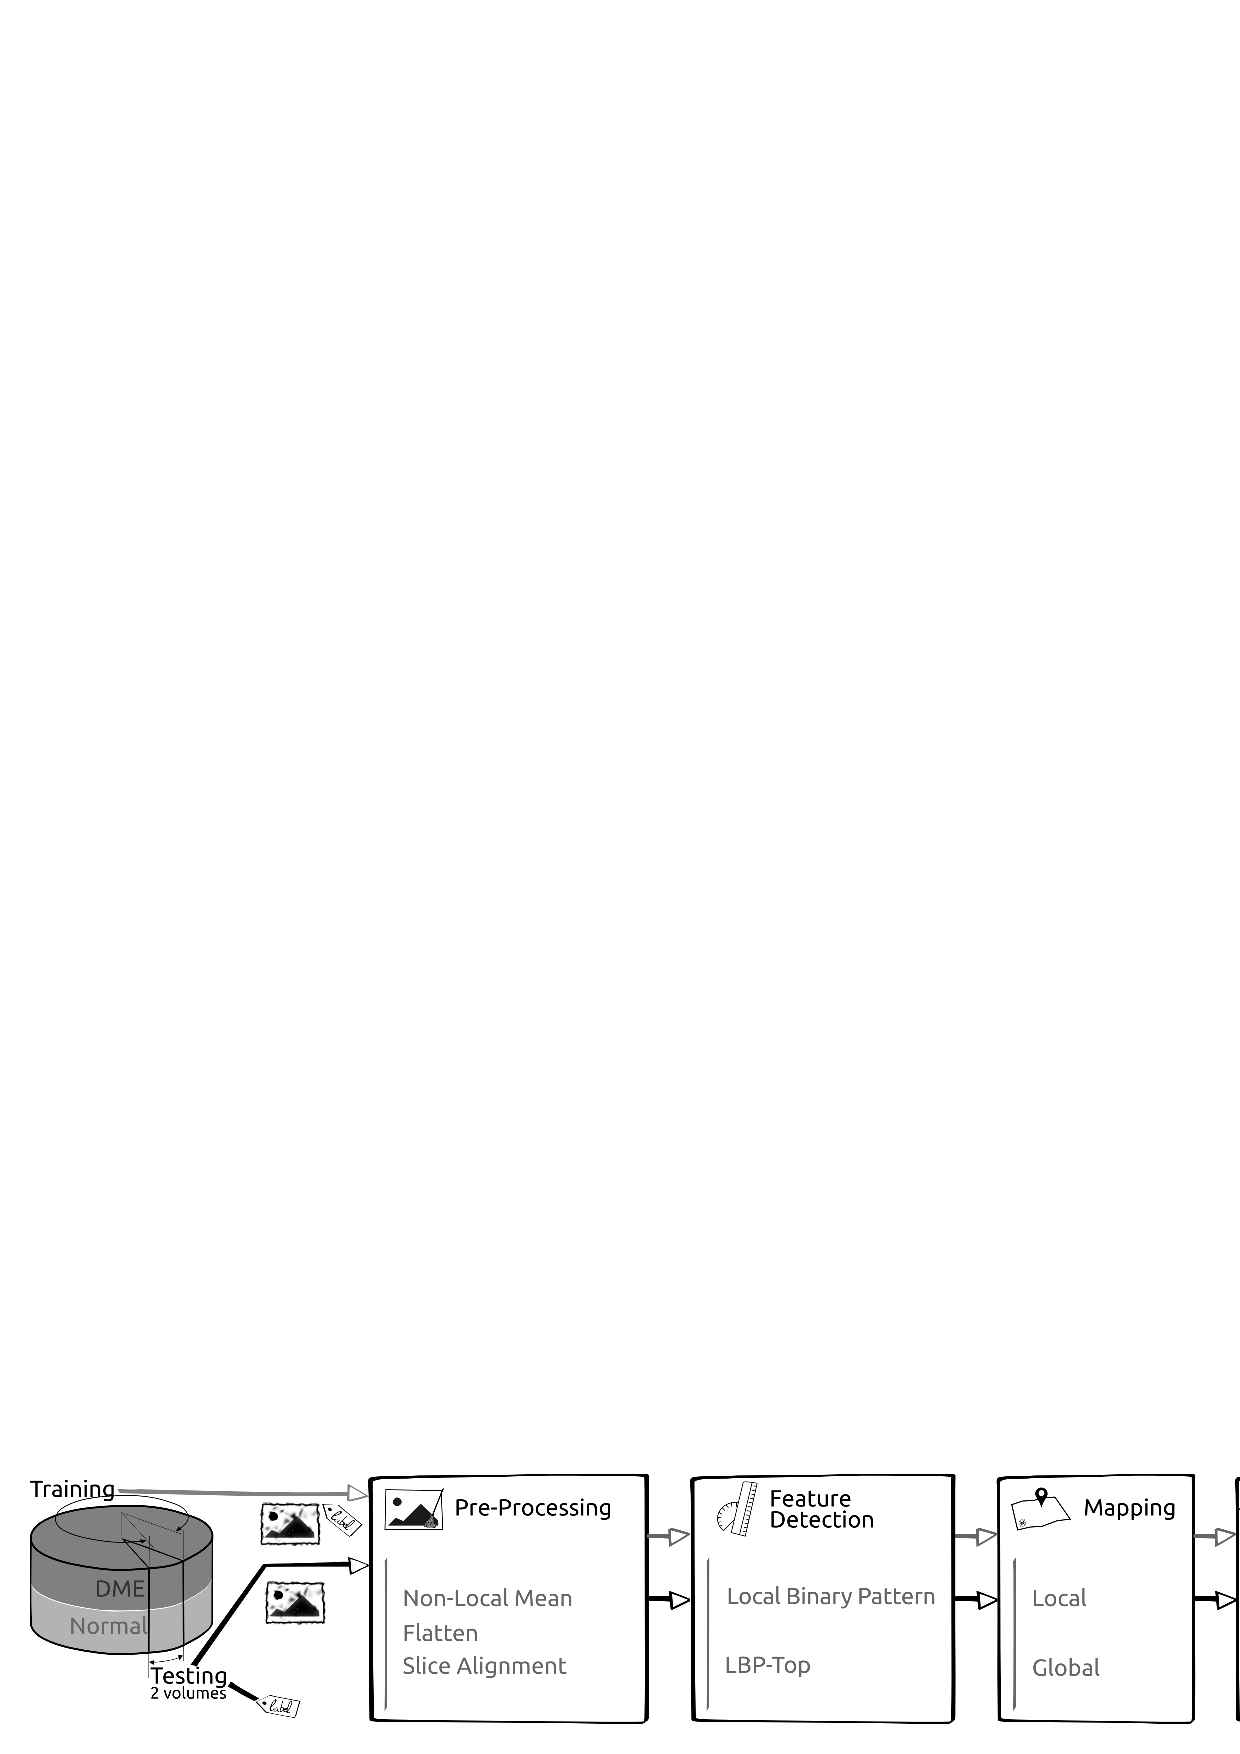
\includegraphics[width=1\linewidth]{content/survey/ml.png}}
    \caption{\added[id=sik]{take out bg crop} Machine learning classification basic scheme}
  \label{fig:ML-scheme}
\end{figure}



\end{landscape}

    % the file wihtout .tex
% include the figures path relative to the master file
% \graphicspath{ {./content/method/figures/visual_cues/}{./content/method/figures/}}
\graphicspath{ {./content/method/figures/}}

\section{Materials and Methods}\label{sec:method}

The proposed method, as well as, its experimental set-up for \ac{oct} volume classification are outlined in Fig.\,\ref{fig:ML-scheme}.
The methodology is formulated as a standard classification procedure which consists of five steps.
First, the \ac{oct} volumes are pre-processed as presented in details in Sect.\,\ref{subsec:prepro}.
Then, \ac{lbp} and \ac{lbptop} features are detected, mapped and represented as discussed in depth in Sect.\,\ref{subsec:feaext}, Sect.\,\ref{subsec:mapping}, and Sect.\,\ref{subsec:fearep}, respectively.
Finally, the classification step is presented in Sect.\,\ref{subsec:cls}.


\subsection{Image pre-processing}\label{subsec:prepro}

This section describes the set of pre-processing techniques which aim at enhancing the \ac{oct} volume.
The influence of these pre-processing methods and their possible combinations are extensively studied in Sect.\,\ref{sec:exp}.

\subsubsection{\acf{nlm}}

\begin{figure}[t]
  \centering
  \hspace*{\fill}
  \subfigure[]{\label{subfig:vol}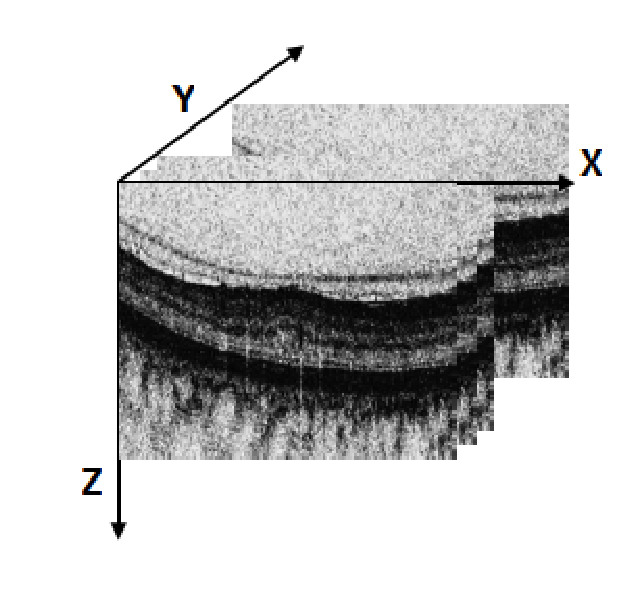
\includegraphics[width=0.3\linewidth]{axs}} \hfill
  \subfigure[]{\label{subfig:raw}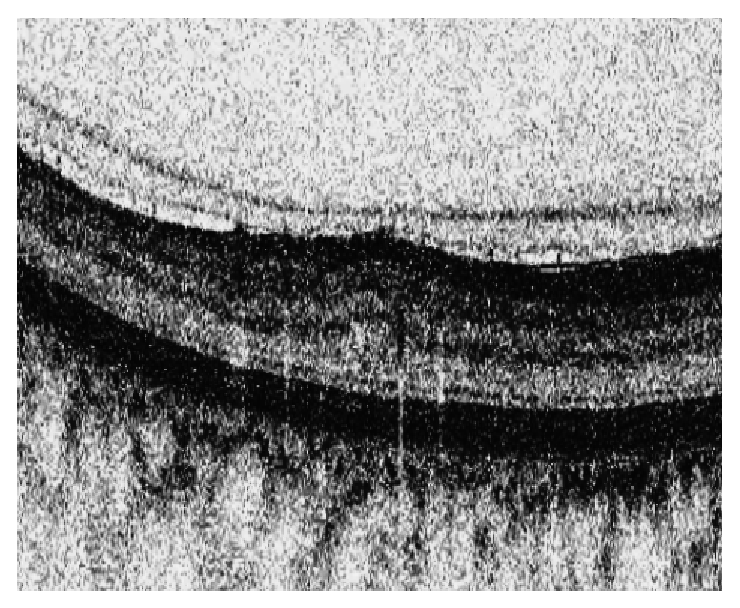
\includegraphics[width=0.3\linewidth]{raw_crop_grey}} \hfill
  \subfigure[]{\label{subfig:nlm}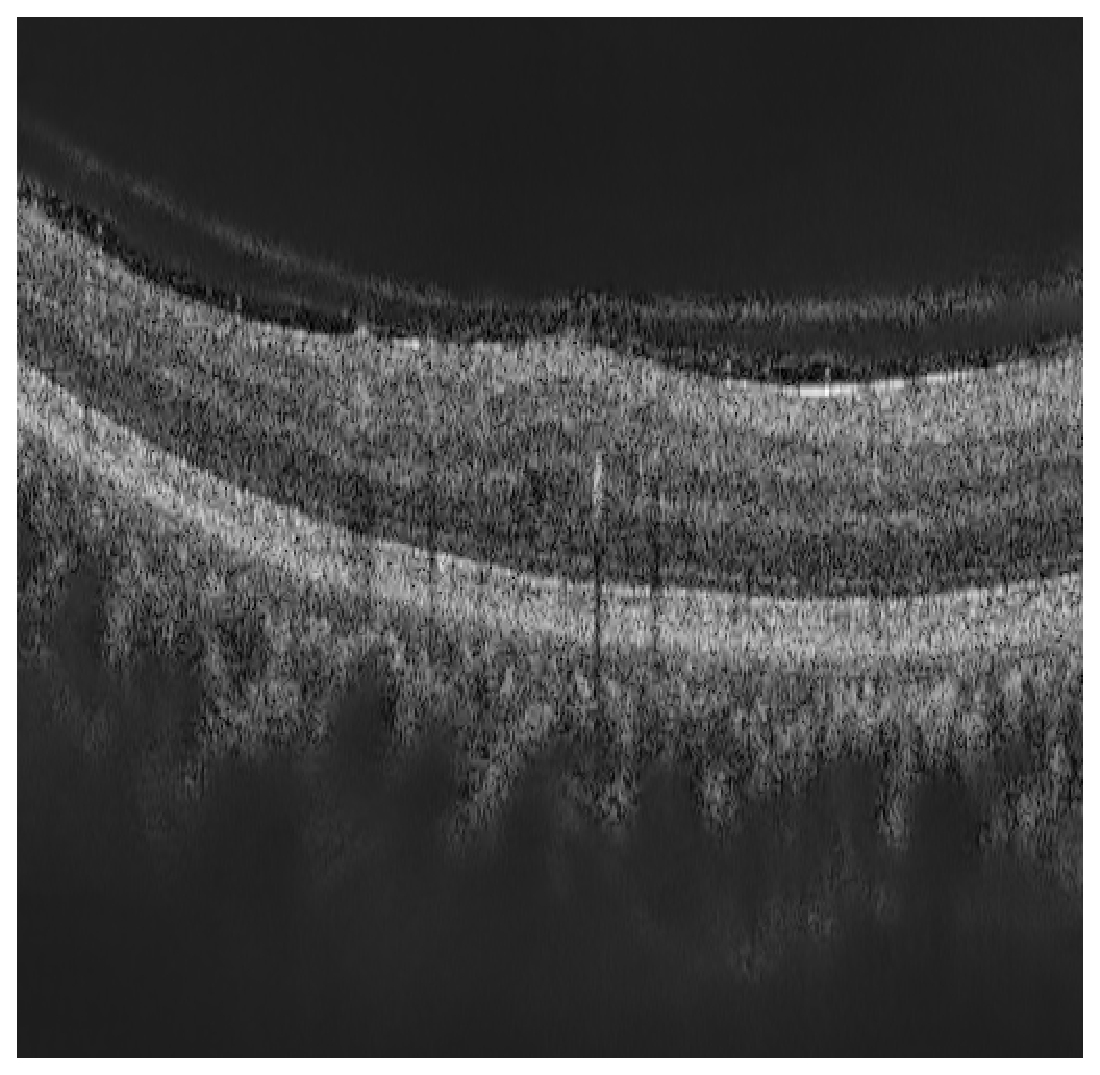
\includegraphics[width=0.3\linewidth]{nlm_crop_grey}}
  \hspace*{\fill}
  \caption{\ac{oct}: (a) Organization of the \ac{oct} data - (b) Original image - (c) \ac{nlm} filtering. Note that the images have been negated for visualization purposes.}
  \label{fig:denoise}
\end{figure}


\ac{oct} images suffer from speckle noise, like other image modalities such as \ac{us}~\cite{schmitt1999speckle}.
The \ac{oct} volumes are enhanced by denoising each B-scan (i.e. each $(x$-$z)$ slice) using the \ac{nlm}~\cite{buades2005non}, as shown in Fig.\,\ref{fig:denoise}.
\ac{nlm} has been successfully applied to \ac{us} images to reduce speckle noise and outperforms other common denoising methods~\cite{Coupe2009}.
\ac{nlm} filtering preserves fine structures as well as flat zones, by using all the possible self-predictions that the image can provide rather than local or frequency filters such as Gaussian, anisotropic, or Wiener filters~\cite{buades2005non}.

\subsubsection{Flattening}

\begin{figure}[t]
\centering 
  \hspace*{\fill}
  \subfigure[]{\label{subfig:flatorg}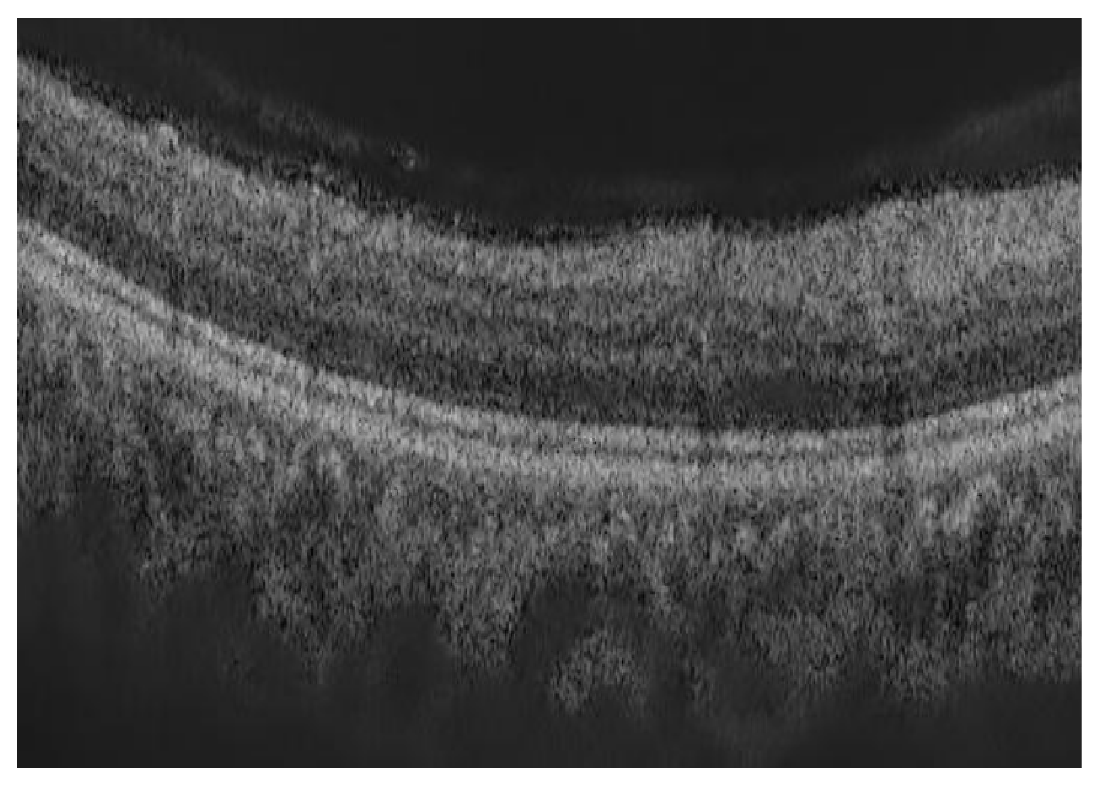
\includegraphics[width=0.20\textwidth]{flattening/original_cropped}}\hfill
  \subfigure[]{\label{subfig:flatotsu}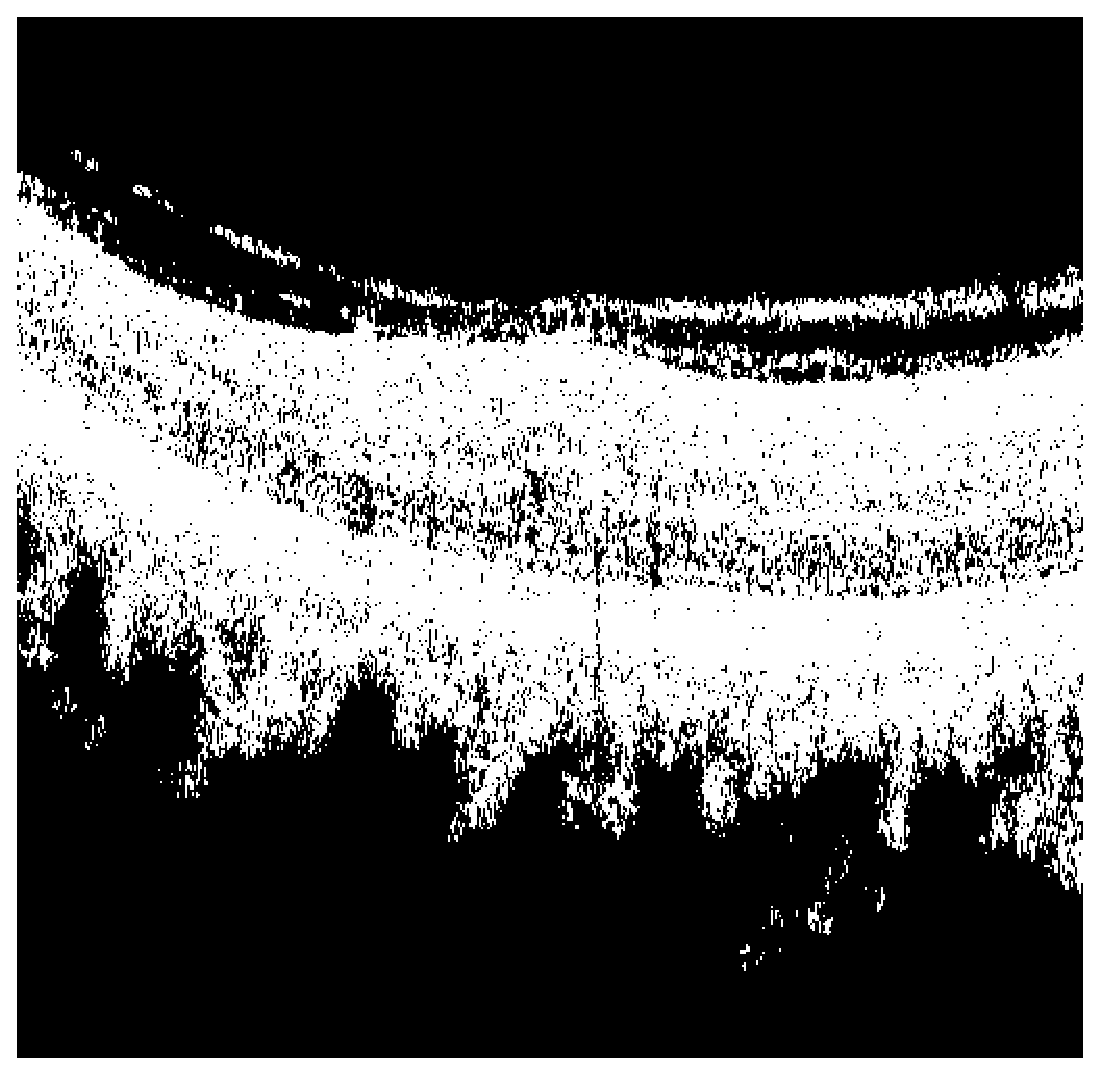
\includegraphics[width=0.20\textwidth]{flattening/thresholding_cropped}}\hfill
  \subfigure[]{\label{subfig:flatmedian}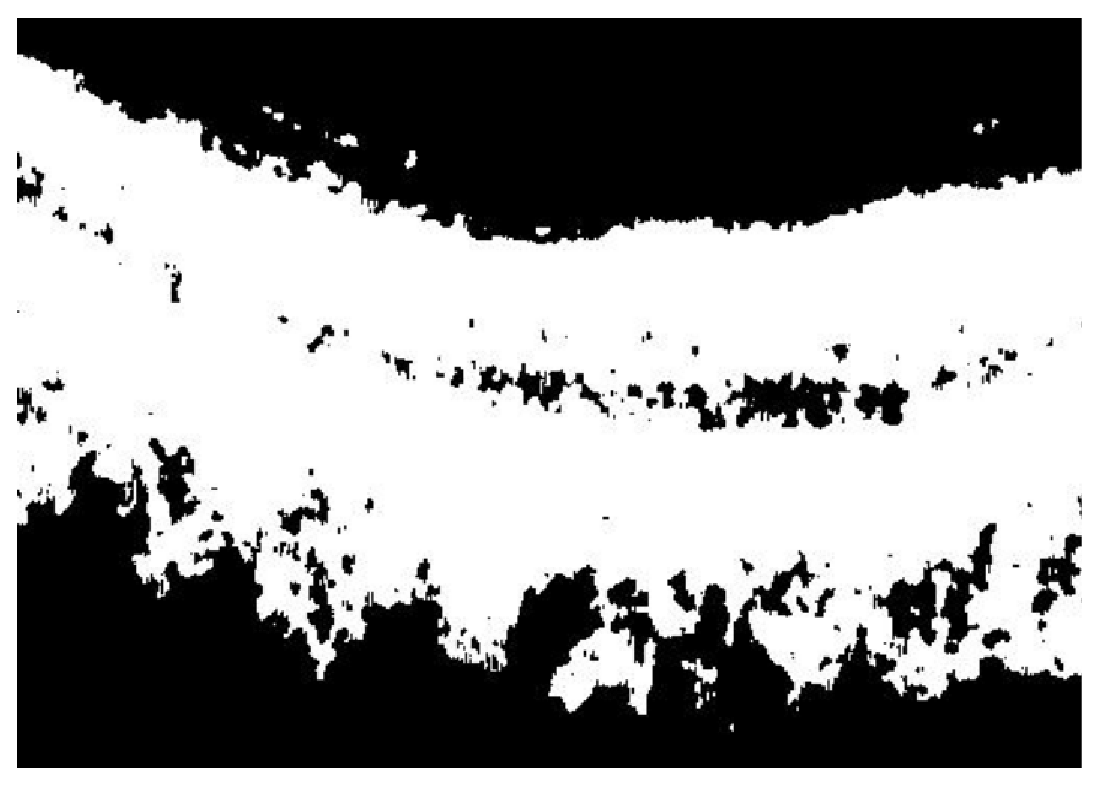
\includegraphics[width=0.20\textwidth]{flattening/median_cropped}}
  \hspace*{\fill}	
  \\
  \hspace*{\fill}
  \subfigure[]{\label{subfig:flatfit}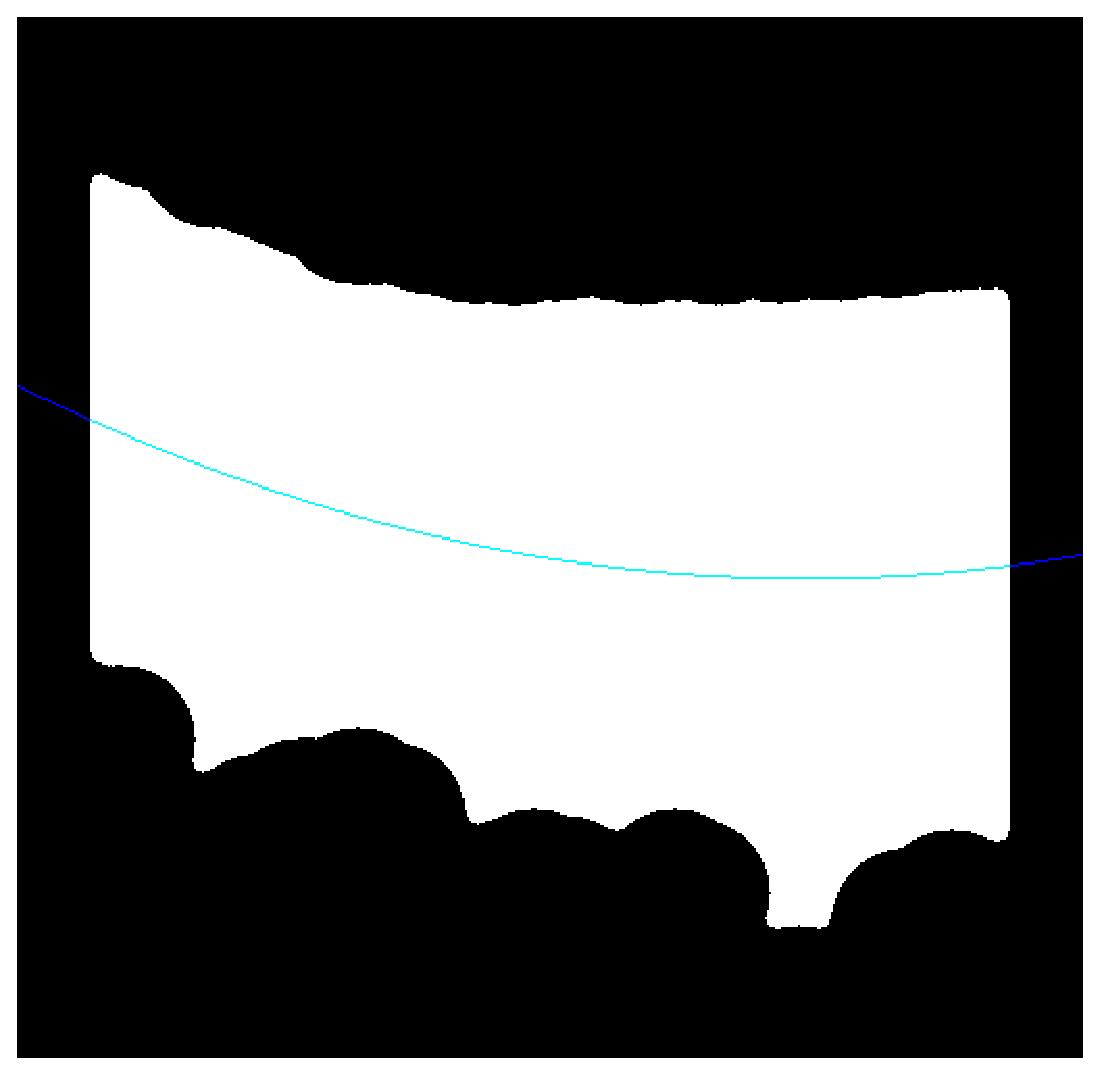
\includegraphics[width=0.20\textwidth]{flattening/fit_cropped}}\hfill
  \subfigure[]{\label{subfig:flatwarp}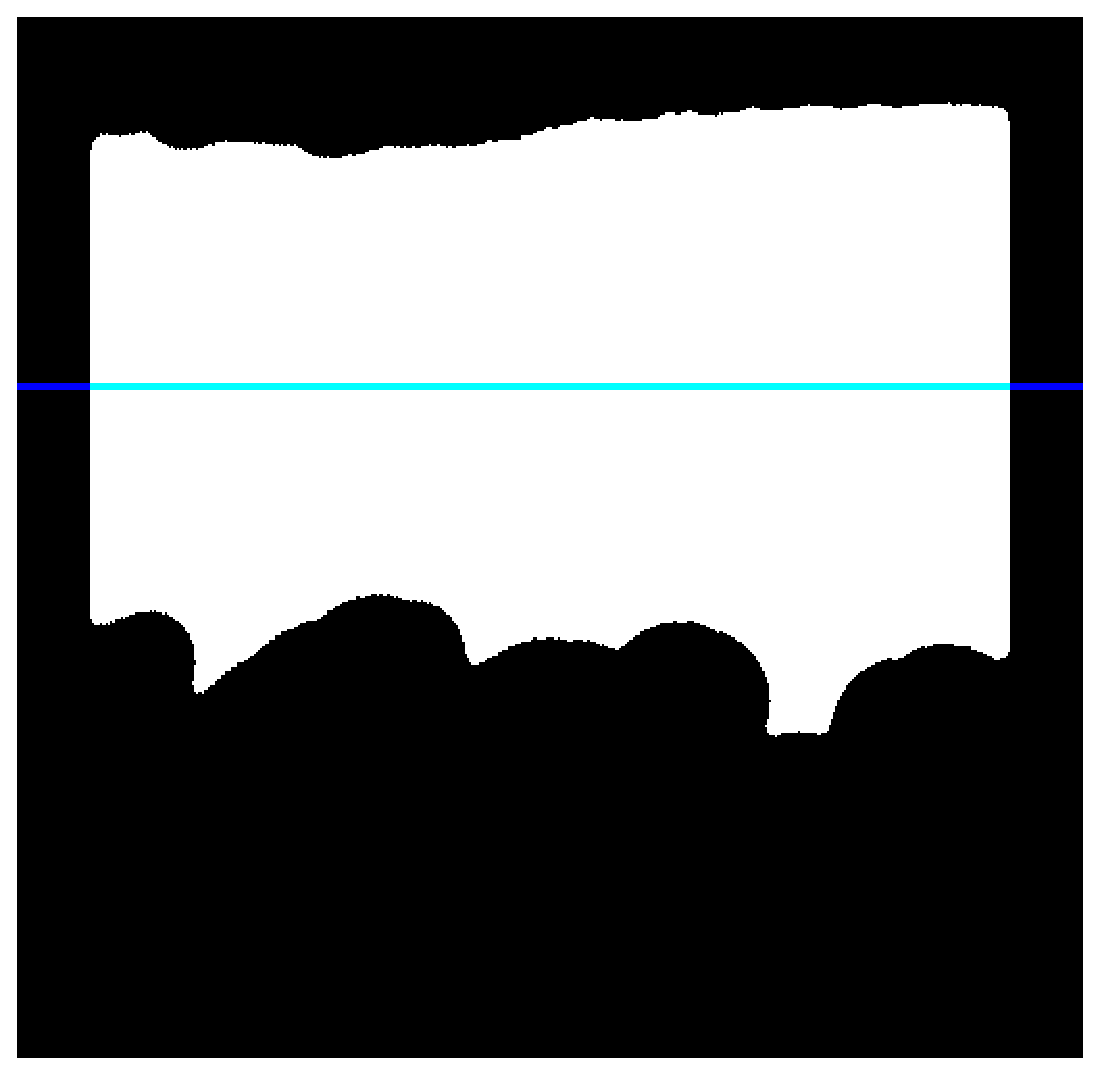
\includegraphics[width=0.20\textwidth]{flattening/warped_cropped}}\hfill
  \subfigure[]{\label{subfig:flatfinal}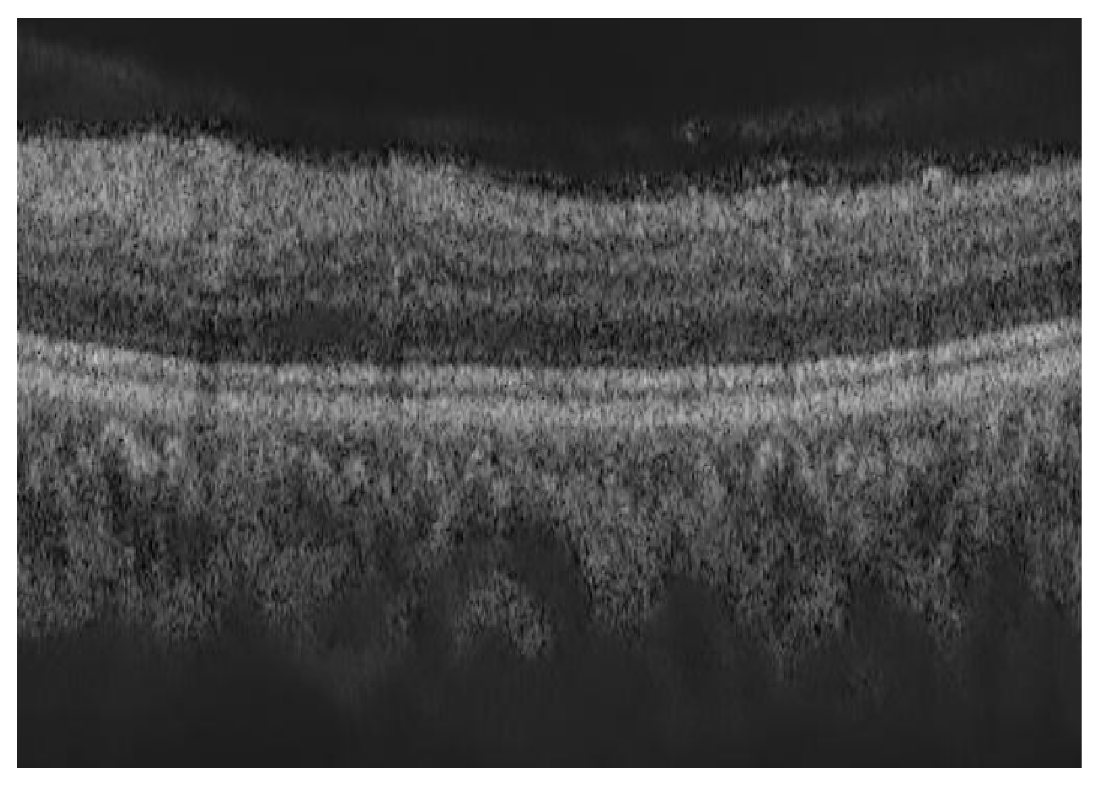
\includegraphics[width=0.20\textwidth]{flattening/warped_org_cropped}}
  \hspace*{\fill}
  \caption{Flattening procedure: (a) original image, (b) thresholding, (c) median filtering, (d) curve fitting, (e) warping, (f) flatten image.}
  \label{fig:flatten}
\end{figure}

Textural descriptors characterize spatial arrangement of intensities.
However, the \ac{oct} scans suffer from large type of variations: inclination angles, positioning, and natural curvature of the retina~\cite{Liu2011}.
Therefore, these variations have to be taken into account to ensure a consistent characterization of the tissue disposition, regardless of the location in the retina.
This invariance can be achieved from different manners: (i) using a rotation invariant descriptor (cf. Sect.\,\ref{subsec:feaext}), or (ii) by unfolding the curvature of the retina.
This latter correction is known as image flattening which theoretically consists of two distinct steps: (i) estimate and fit the curvature of the \ac{rpe} and (ii) warp the \ac{oct} volume such that the \ac{rpe} becomes flat.

Our correction is similar to the one of Liu\,\textit{et~al.}~\cite{Liu2011}: each B-scan is thresholded using Otsu's method followed by a median filtering to detect the different retina layers (see Fig\,\ref{subfig:flatmedian} and Fig\,\ref{subfig:flatotsu}). 
Then, a morphological closing and opening is applied to fill the holes and the resulting area is fitted using a second-order polynomial (see Fig.\,\ref{subfig:flatfit}). 
Finally, the scan is warped such that the curve becomes a line as presented in Fig.\,\ref{subfig:flatwarp} and Fig.\,\ref{subfig:flatfinal}. 

\subsubsection{Slice alignment}
The flattening correction does not enforce an alignment through the \ac{oct} volume.
Thus, in addition to the flattening correction, the warped curves of each B-scan are positioned at the same altitude in the $z$ axis. 

\subsection{Feature detection}\label{subsec:feaext}
In this research, we choose to detect simple and efficient \ac{lbp} texture features with regards to each \ac{oct} slice and volume.
\ac{lbp} is a texture descriptor based on the signs of the differences of a central pixel with respect to its neighboring pixels~\cite{ojala2002multiresolution}.
These differences are encoded in terms of binary patterns as in~Eq.\,\eqref{Eq:LBP}:

\begin{equation}\label{Eq:LBP}
LBP_{P,R} = \sum_{p=0}^{P-1}s(g_{p} - g_{c})2^{p} \ , \qquad s(x) = \begin{cases}
    1  & \ \text{if } x \geq 0\\
    0  & \ \text{otherwise}\\
  \end{cases} \ ,
\end{equation}

\noindent where $g_c$, $g_{p}$ are the intensities of the central pixel and a given neighbor pixel, respectively; $P$ is the number of sampling points in the circle of radius $R$.

Ojala\,\textit{et~al.} further extended the original \ac{lbp} formulation to achieve rotation invariance at the expense of limiting the texture description to the notion of circular ``uniformity''~\cite{ojala2002multiresolution}.
Referring to the coordinate system defined in Fig.\,\ref{subfig:vol}, the \ac{lbp} codes are computed on each $(x$-$z)$ slice, leading to a set of \ac{lbp} maps, a map for each $(x$-$z)$ slice.

Volume encoding is later proposed by Zhao\,\textit{et~al.} by computing \ac{lbp} descriptors in three orthogonal planes, so called \ac{lbptop}~\cite{zhao2012rotation}.
More precisely, the \ac{lbp} codes are computed considering the $(x$-$z)$ plane, $(x$-$y)$ plane, and $(y$-$z)$ plane, independently.
Thus, three sets of \ac{lbp} maps are obtained, one for each orthogonal plane.

In this work, we consider rotation invariant and uniform \ac{lbp} and \ac{lbptop} features with various sampling points (i.e., $\{8,16,24\}$) with respect to different radius, (i.e., $\{1,2,3\}$).
The number of patterns ($LBP_{\#pat}$) in regards with each configuration is reported in Table~\ref{tab:lbphist}.

\begin{table}
\caption{Number of patterns ($LBP_{\#pat}$) for different sampling points and radius ($\{P,R\}$) of the \ac{lbp} descriptor.}
\centering{
\resizebox{0.5\linewidth}{!}{
\footnotesize{
\begin{tabular}{l  c c c }
\toprule
 \multicolumn{4}{c}{Sampling point for a radius ($\{P, R\}$)}\\
 \midrule
 & $\{8, 1\}$ & $\{16, 2\}$ & $\{24, 3\}$\\
 \cmidrule{2-4}
  $LBP_{\#pat}$  & 10 & 18 & 26 \\
 \bottomrule
\end{tabular}}}}
\label{tab:lbphist}
\end{table}

\subsection{Mapping} \label{subsec:mapping}
The mapping stage is used to partition the previously computed \ac{lbp} maps; for this work, two mapping strategies are defined: (i) \emph{global} and (ii) \emph{local} mapping.
The size of the feature descriptor is summarized in Table~\ref{tab:descsize}.

\begin{table}
\caption{Size of a descriptor for an \ac{sdoct} volume. $d$ denotes the number of slices in the volume, $N$ the number of 2D windows, and $N'$ the number of 3D sub-volumes, respectively.}
\centering{
\footnotesize{
\begin{tabular}{l c c }
  \ctoprule{2-3}
  & Global mapping & Local mapping \\
  \midrule
  \ac{lbp} & $d \times LBP_{\#pat}$ & $(N \times d) \times LBP_{\#pat}$ \\
  \midrule
  \ac{lbptop} & $1 \times (3 \times LBP_{\#pat})$ & $N' \times (3 \times LBP_{\#pat})$ \\
  \bottomrule
\end{tabular}}}
\label{tab:descsize}
\end{table}

\begin{figure}[t]
  \centering
  \hspace*{\fill}
  \subfigure[]{\label{subfig:glbp}
\includegraphics[width=0.25\linewidth]{global-lbp}} \hfill
  \subfigure[]{\label{subfig:glbptop}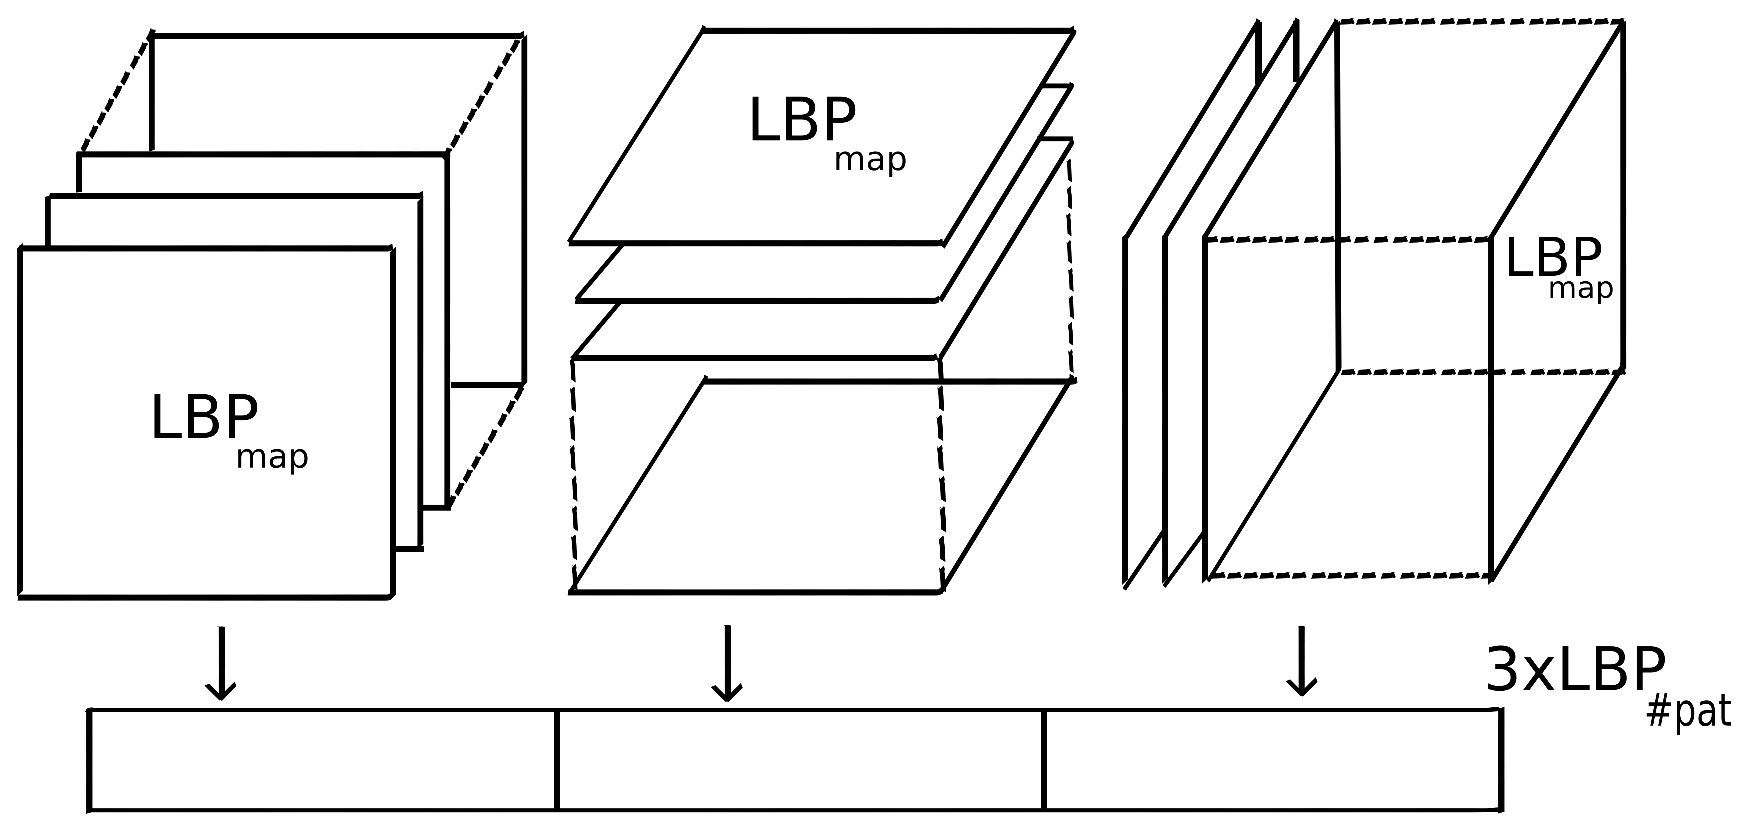
\includegraphics[width=0.48\linewidth]{global-lbptop}}
  \hspace*{\fill}\\
  \hspace*{\fill}
  \subfigure[]{\label{subfig:llbp}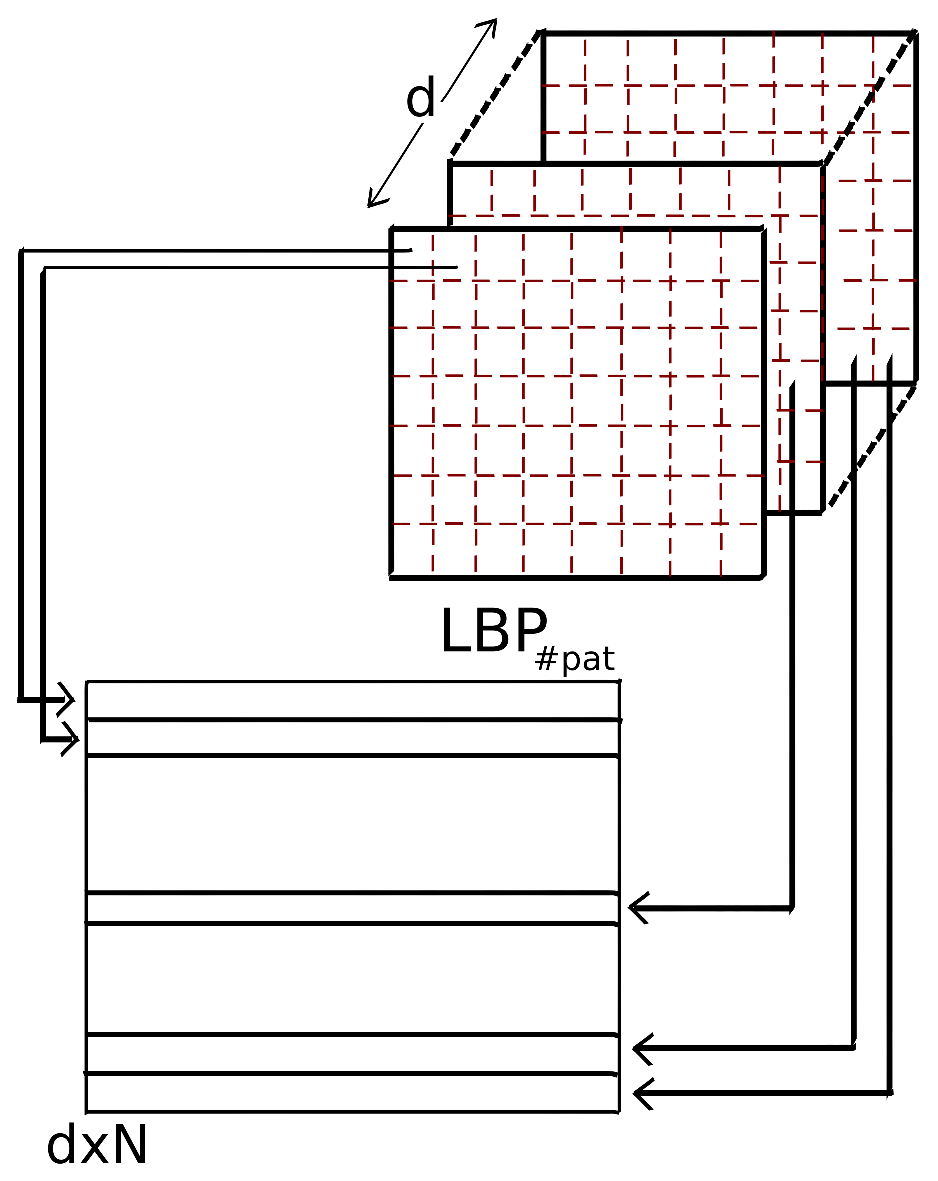
\includegraphics[width=0.25\linewidth]{local-lbp}} \hfill
  \subfigure[]{\label{subfig:llbptop}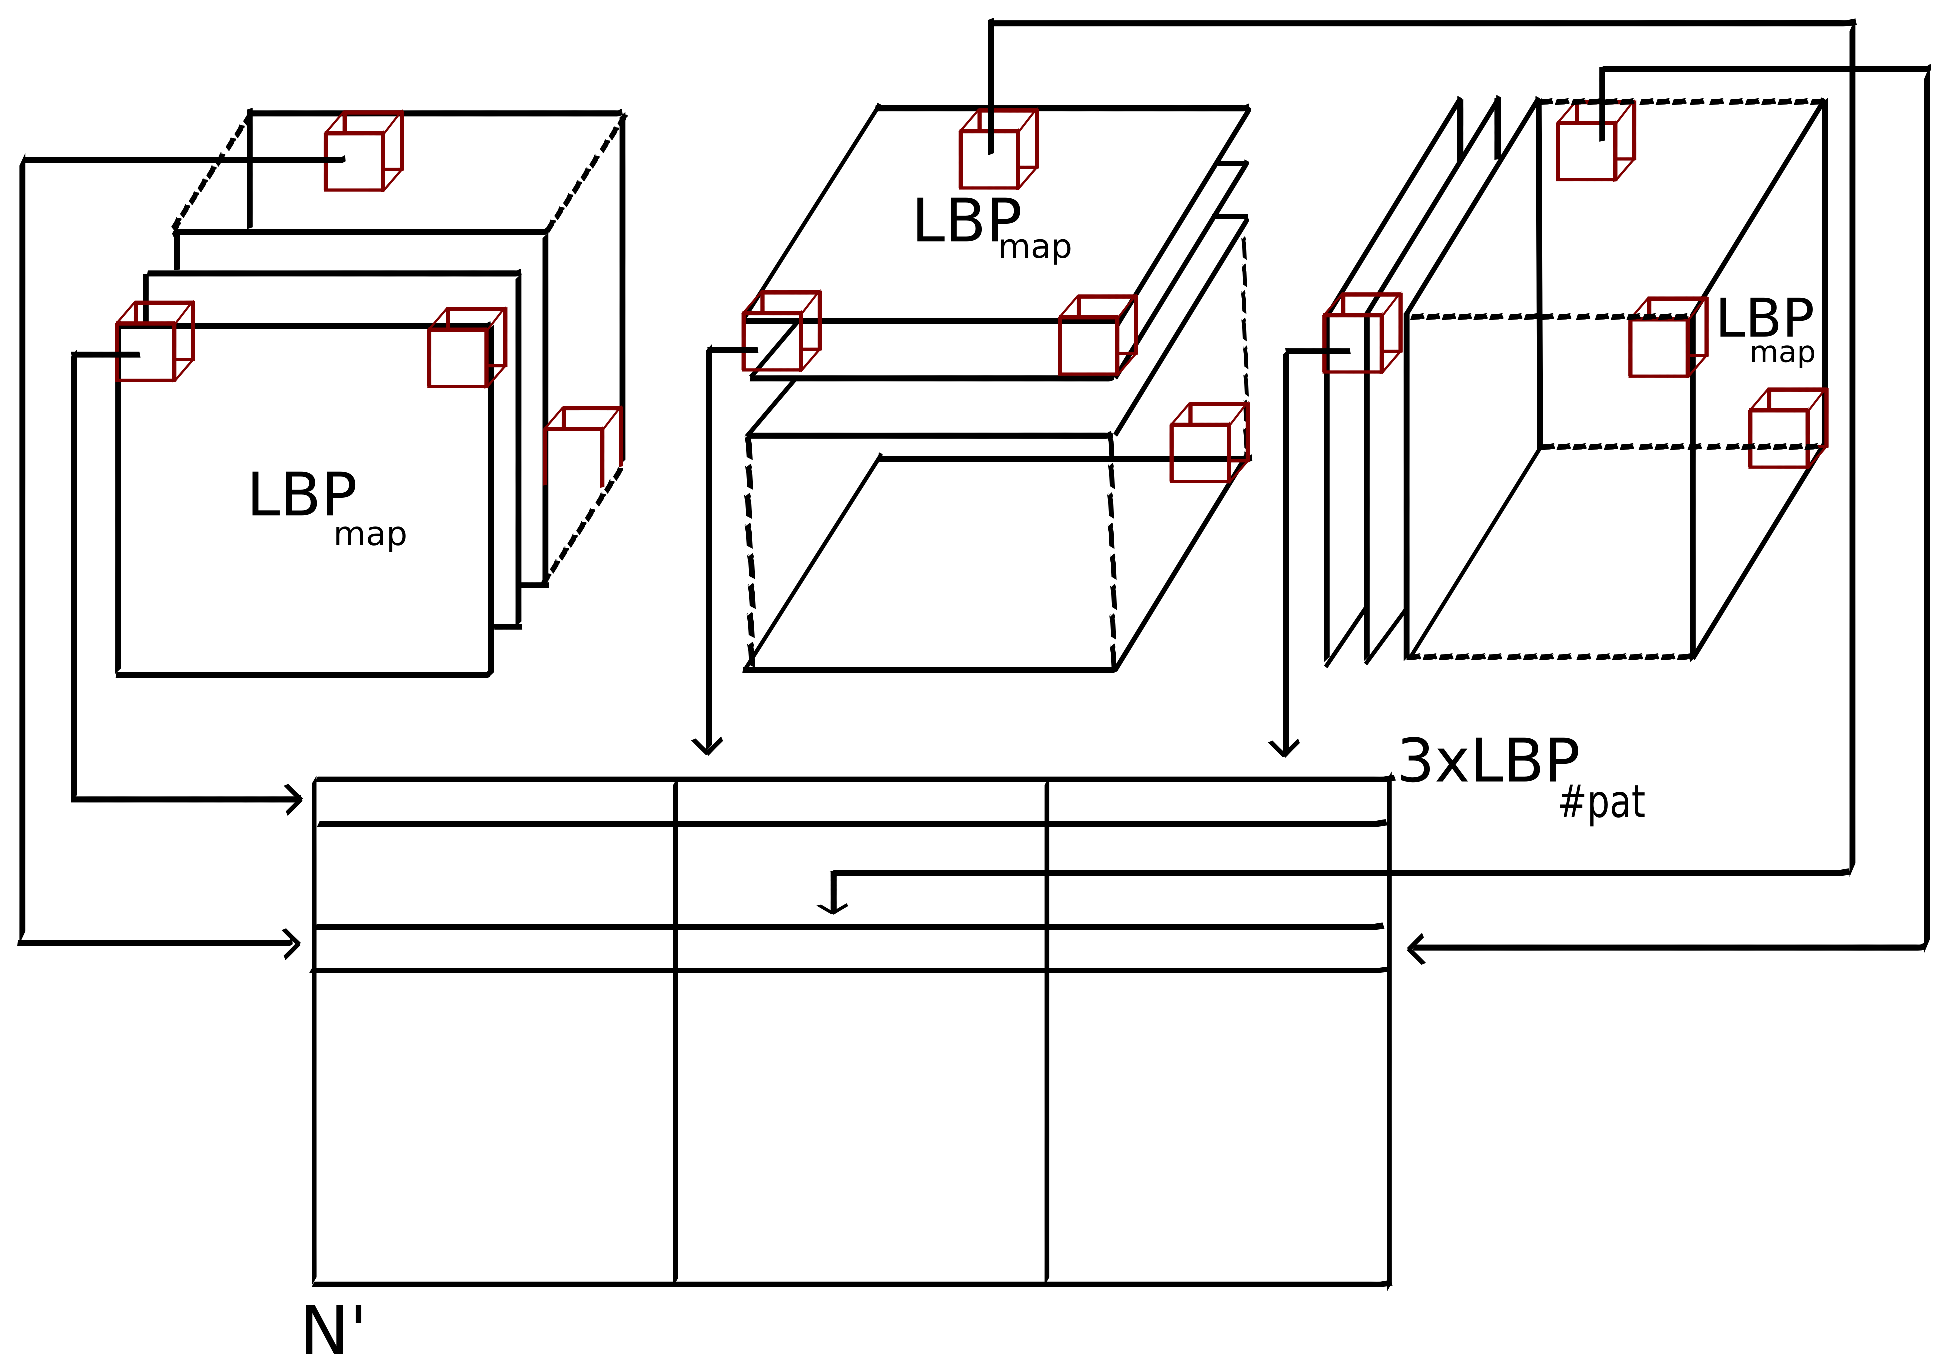
\includegraphics[width=0.48\linewidth]{local-lbptop}}
  \hspace*{\fill}
  \caption{Graphical representation of the feature extraction: (a) extraction of \ac{lbp} for global mapping - (b) extraction of \ac{lbptop} for global mapping - (c) extraction of \ac{lbp} for local mapping - (d) extraction of \ac{lbptop} for local mapping.}
  \label{fig:feaextimg}
\end{figure}

\begin{description}
\item[\emph{Global}] mapping extracts the final descriptors from the 2D feature image for \ac{lbp} and 3D volume for \ac{lbptop}.
%mapping considers to extract the features from the 2D B-scans for \ac{lbp} and 3D volume for \ac{lbptop}.
Therefore, for a volume with $d$ slices, the \emph{global}-\ac{lbp} mapping will lead to the extraction of $d$ elements.
While the \emph{global}-\ac{lbptop} represents the whole volume as a single element.
The \emph{global} mapping for 2D images and 3D volume is shown in Fig.~\ref{subfig:glbp} and \ref{subfig:glbptop}.

\item[\emph{Local}] mapping extracts the final descriptors from a set of ($m \times m$) 2D patches for \ac{lbp} and a set of ($ m \times m \times m$) sub-volumes for \ac{lbptop}.
Given $N$ and $N'$ the total number of 2D patches and 3D sub-volumes respectively, the \emph{local}-\ac{lbp} approach provides $N \times d$ elements, while \emph{local}-\ac{lbptop} provides $N'$ elements.
%Here $N$ and $N'$ are the total number of elements per B-scane or the volume, respectively.
This mapping is illustrated in Fig.~\ref{subfig:llbp} and \ref{subfig:llbptop}.

\end{description}

\subsection{Feature representation}\label{subsec:fearep}

Two strategies are used to describe each \ac{oct} volume's texture.

\begin{description}

\item[Low-level representation] The texture descriptor of an \ac{oct} volume is defined as the concatenation of the \ac{lbp} histograms with the \emph{global}-mapping.
The \ac{lbp} histograms are extracted from the previously computed \ac{lbp} maps (see Sect.\,\ref{subsec:feaext}).
Therefore, the \ac{lbptop} final descriptor is computed through the concatenation of the \ac{lbp} histograms of the three orthogonal planes with the final size of $3 \times LBP_{\#pat}$.
More precisely, an \ac{lbp} histogram is computed for each set of \ac{lbp} maps $(x$-$z)$ plane, $(x$-$y)$ plane, and $(y$-$z)$ plane, respectively.
Similarly, the \ac{lbp} descriptor is defined through concatenation of the \ac{lbp} histograms per each $(x$-$z)$ slice with the final size of $d \times LBP_{\#pat}$.

\item[High-level representation] The concatenation of histograms employed in the low-level representation in conjunction with either \emph{global}- or \emph{local}-mapping can lead to a high dimensional feature space.
For instance, \emph{local}-mapping results in a size of $N \times d \times LBP_{\#pat}$ for the final \ac{lbp} descriptor and $N' \times LBP_{\#pat}$ for the final \ac{lbptop} descriptor, where $N$ and $N'$ are the total number of 2D patches and 3D sub-volumes, respectively.
High-level representation simplifies this high dimensional feature space into a more discriminant lower space.
\ac{bow} approach is used for this purpose~\cite{Sivic2003}.
This model represents the features by creating a codebook or visual dictionary, from the set of low-level features.
The set of low-level features are clustered using \textit{k}-means to create the codebook with \textit{k} clusters or visual words.
After creating the codebook from the training set, the low-level descriptors are replaced by their closest word within the codebook.
The final descriptor is a histogram of size \textit{k} which represents the codebook occurrences for a given mapping.

\end{description}

\subsection{Classification}\label{subsec:cls}

The last step of our framework consists in the classification of \ac{sdoct} volumes as normal or \ac{dme}.
For that matter, five different classifiers are used: (i) $k$-\acf{nn}, (ii) \acf{lr}~\cite{cox1958regression}, (iii) \acf{rf}~\cite{breiman2001random}, (iv) \acf{gb}~\cite{friedman2002stochastic, lemaitre2015boosting}, and (v) \acf{svm}~\cite{vapnik1963generalized, aizerman1964}.
Details regarding the parameters used in our experiments are provided in Sect.\,\ref{sec:exp}.

%%% Local Variables:
%%% mode: latex
%%% TeX-master: "../../main.tex"
%%% End:

% % include the figures path relative to the master file
 \graphicspath{ {./content/experiment/figures/} }

\section{Experiments}
\label{sec:exp}

% The aim of this work is to stress some of the design choices done in
% \cite{Lemaintre2015miccaiOCT}, further test the influence of the new blocks
% composing our framework and compare in comparison to its earlier version.

This section describes the conceived experimentation to investigate the effects
of (i) optimal number of words, (ii) different pre-processing steps, and (iii)
different classifiers.
Table~\ref{tab:experiment_summary} reports the experimentation
in~\cite{Lemaintre2015miccaiOCT} as a baseline, and outlines the complementary
experimentation here proposed.
The reminder of this section details experiment commonalities, while experiment particularities are reported in the following subsections, and a complete set of the results obtained at each experiment is found in Appendix~\ref{app:1}.

All the experiments are performed using our own dataset reported in Sect.\,\ref{sec:exp:dataset:seri} and reported according to Sect.\,\ref{sec:exp:eval}.
\ac{lbp} and \ac{lbptop} features are extracted for different sampling points of 8, 16, and 24 for radius of 1, 2, and 3, respectively.
Both \emph{local}- and \emph{global}-mapping strategies are used when applicable.
The partitioning for \emph{local}-mapping is set to ($7 \times 7$) patch for 2D \ac{lbp} and ($ 7 \times 7 \times 7$) sub-volume for \ac{lbptop}.

\begin{landscape}
  \begin{table}[ht]
\caption{The outline and summary of the performed experiments.}
\medskip
\scriptsize{
\begin{center}
\resizebox{1\linewidth}{!}{
\begin{tabular}{l  c	 c  c  c  c  c  c  c }
\toprule
\\
&  Dataset & Pre-processing & Features & Mapping & Representation & Classification & Validation & Evaluation \\
\cmidrule(l){2-9}
\\
\multirow{3}{*}{Common:} & \multirow{3}{*}{SERI} & \multirow{3}{*}{\ac{nlm}} & \ac{lbp},\ac{lbptop} & \multirow{3}{*}{} & \multirow{3}{*}{}  & & \multirow{3}{*}{\ac{lopocv}}& \multirow{3}{*}{} \\
        &      &          & $S = \{8,16,24\}$ & & & & & \\
        &      &          & $R = \{1,2,3\}$  & & & & & \\\\
\midrule
\\
Experiment\#1:  \\
%\hdashline \noalign{\vskip 3pt}
%\\
\multirow{2}{4cm}{Goal: Evaluation of features, mapping and representation} & \multirow{2}{*}{+ Duke} &\multirow{2}{*}{$\sim$} & \multirow{2}{*}{$\sim$} & \emph{global} & \ac{bow} & \multirow{2}{*}{\ac{rf}} & \multirow{2}{*}{$\sim$} & \multirow{2}{*}{\ac{se}, \ac{sp}, \cite{Venhuizen2015}}\\
&  & & & \emph{local} & Histogram &  & & \\\\
\midrule
\\
Experiment\#2:\\
%\hdashline \noalign{\vskip 3pt}
%\\
\multirow{2}{4cm}{Goal: Finding the optimum number of words}& \multirow{2}{*}{$\sim$} & + \acs{f} & \multirow{2}{*}{$\sim$} & \emph{global} & \multirow{2}{*}{\ac{bow}} & \multirow{2}{*}{\ac{lr}} & \multirow{2}{*}{$\sim$} & \multirow{2}{*}{ \ac{acc}, \ac{f1}}\\
  & & + \acs{fal} & & \emph{local} & & & & \\\\
\midrule
\\
Experiment\#3: \\
%\hdashline \noalign{\vskip 3pt}
%\\
%\hdashline \noalign{\vskip 3pt}
 \multirow{4}{4cm}{Goal: Evaluation of different pre-processing for high-level features }& \multirow{4}{*}{$\sim$} & \multirow{2}{*}{+\acs{f}} & \multirow{4}{*}{$\sim$} & \multirow{2}{*}{\emph{global}} & \multirow{4}{*}{\ac{bow}} & $3$-\ac{nn} & \multirow{4}{*}{$\sim$} & \multirow{4}{*}{\ac{se}, \ac{sp}}\\
 & & \multirow{2}{*}{+\acs{fal}} & & \multirow{2}{*}{\emph{local}} &  & \ac{rf} & & \\
 & & & & & & \ac{svm} & & \\
 & & & & & & \ac{gb} & & \\
\midrule
\\
Experiment\#4:\\
%\hdashline \noalign{\vskip 3pt}
%\\
%\hdashline \noalign{\vskip 3pt}
\multirow{4}{4cm}{Goal: Evaluation of different pre-processing for low-level features} & \multirow{4}{*}{$\sim$} & \multirow{2}{*}{ +\acs{f}} & \multirow{4}{*}{$\sim$} & \multirow{4}{*}{\emph{global}} & \multirow{4}{*}{Histogram} & $3$-\ac{nn} & \multirow{4}{*}{$\sim$} & \multirow{4}{*}{\ac{se}, \ac{sp}}\\
& & \multirow{2}{*}{+\ac{fal}} & & & & \ac{rf} &  &\\
& & & & & & \ac{svm} & & \\
& & & & & & \ac{gb} & & \\
\\
\bottomrule


\end{tabular}}
\end{center}}
\label{tab:table4}
\end{table}
\end{landscape}


\subsection{Dataset}\label{sec:exp:dataset:seri}
This data was acquired by the Singapore Eye Research Institute (SERI), using CIRRUS TM (Carl Zeiss Meditec, Inc., Dublin, CA) \ac{sdoct} device. The datasets consist of 32 \ac{oct} volumes (16 \ac{dme} and 16 normal cases). Each volume contains 128 B-scan with resolution of 512 $\times$ 1024 pixels.
All \ac{sdoct} images are read and assessed by trained graders and identified as normal or \ac{dme} cases based on evaluation of retinal thickening, hard exudates, intraretinal cystoid space formation and subretinal fluid.

\subsection{Evaluation}\label{sec:exp:eval}
Accordingly to~\cite{Lemaintre2015miccaiOCT}, all the experiments are evaluated in terms of \acf{se} and \acf{sp} using \ac{lopocv} strategy.

\ac{se} and \ac{sp} are statistics driven from the confusion matrix (see Fig.\,\ref{fig:CM}) as stated in Eq.\,\ref{eq:sesp}.
The \ac{se} evaluates the performance of the classifier with respect to the positive class, while the \ac{sp} evaluates its performance with respect to negative class.

\begin{figure}
\begin{center}
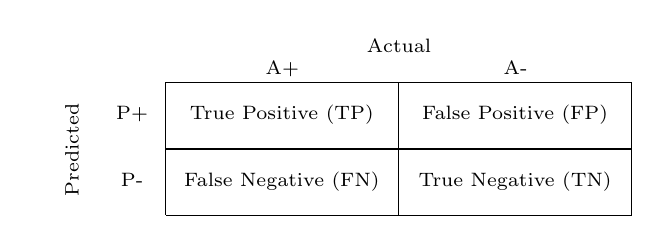
\begin{tikzpicture}[scale=0.4]
      \node at (1,1){
      \scriptsize{
        \begin{tabular}{
            >{\centering}m{1em} >{\centering}m{1em} >{\centering}m{1in} >{\centering\arraybackslash}m{1in}}
          % c>{\centering}m{2em}ccc}
          & & \multicolumn{2}{c}{ Actual}\\
          & & A+ & A- \\
          \cline{3-4}
          & \multicolumn{1}{c|}{} & \multicolumn{1}{c|}{} & \multicolumn{1}{c|}{}\\
          \multirow{3}{*}{\rotatebox[origin=c]{90}{Predicted}}& \multicolumn{1}{c|}{P+} &  \multicolumn{1}{c|}{True Positive (TP)} & \multicolumn{1}{c|}{False Positive (FP)} \\
          &\multicolumn{1}{c|}{}  & \multicolumn{1}{c|}{}& \multicolumn{1}{c|}{} \\
          \cline{3-4}
          & \multicolumn{1}{c|}{} &\multicolumn{1}{c|}{} & \multicolumn{1}{c|}{}\\

          & \multicolumn{1}{c|}{P-} &\multicolumn{1}{c|}{False Negative (FN)}  &\multicolumn{1}{c|}{True Negative (TN)}\\
          & \multicolumn{1}{c|}{} &\multicolumn{1}{c|}{} & \multicolumn{1}{c|}{}\\
          \cline{3-4}
          \end{tabular}
      }};
    \end{tikzpicture}
    \end{center}
\caption{Confusion matrix with true and false positive detected samples (\acs{tp}, \acs{fp}) in the first row, from left to right and the false and true negative detected samples (\acs{fn}, \acs{tn}) in the second row, from left to right.}
\label{fig:CM}
\end{figure}

\begin{align}
 \ac{se}  = \frac{TP}{TP+FN} \qquad \ac{sp} = \frac{TN}{TN+FP}
 \label{eq:sesp}
\end{align}

The usage of \ac{lopocv} implies that at each round, a pair \ac{dme}-normal volume is selected for testing while the remaining volumes are used for training.
Subsequently, no \ac{se} or \ac{sp} variance can be reported.
However, \ac{lopocv} strategy has been adopted despite this limitation due to the reduced size of the dataset.

\subsection{Experiment \#1: \acs{bow} dictionary size}\label{subsec:exp1}
% Experiment structure
%
% Intro:
%   - background
%   - goal / experiment intention / why
%   - data
%   - evaluation
%   - reference to result table
%
% Procedure (by data if more than one):
%   - pre-processing
%   - feature extraction
%   - mapping
%   - feature representation
%   - classifier
%
% Remarks (if any)
%
% Result highlights:
%   - (only a description)

%% Experiment intro
On its original implementation~\cite{Lemaitre2015, Lemaintre2015miccaiOCT} the codebook size was arbitrarily set $k=32$.
This experiment evaluates several codebook sizes to find optimal size of the codebook in variated conditions.

%% Experiment procedure
Several pre-processing strategies are evaluated: (i) \nlm, (ii) a combination of \nlm and flattening, and (iii) a combination of \nlm, flattening and aligning.
\lbp and \lbptop descriptors are detected using the default configuration.
Volumes are represented using \ac{bow}, where the codebook size ranging for $k \in \{10, 20, 30, \cdots, 100, 200, \cdots, 500, 1000\}$.
Finally, the volumes are classified using \lr.
The choice of this linear classifier avoids that the results get boosted by the classifier. In this manner any improvement would be linked to the pre-processing and the size of the codebook.
%
\begin{landscape}
  \begin{table}
\caption{Experiment \#1 - Optimum number of words for each configuration as a result of \ac{lr} Classification, for high-level feature extraction of \emph{global} and \emph{local}-\ac{lbp}, and \emph{local}-\ac{lbptop} features with different pre-processing. The pre-processing includes: \ac{nf}, \ac{f}, and \ac{fal}.
The achieved performances are indicated in terms of  \acs{acc}, \acs{f1}, \acs{se}, and \acs{sp}}
\centering

\footnotesize{
\resizebox{1\linewidth}{!}{
\begin{tabular}{ll  ccccr	c	ccccr	c ccccr}
\toprule
Features & Pre-processing &    \multicolumn{5}{c}{$\{8,1\}$}  & & \multicolumn{5}{c}{$\{16,2\}$} & & \multicolumn{5}{c}{$\{24,3\}$} \\
  \cmidrule(l){3-7}  \cmidrule(l){9-13}  \cmidrule(l){15-19}
   & &  	\ac{acc}\% & \ac{f1}\% & \ac{se}\% & \ac{sp}\%  & W\# &  & \ac{acc}\% & \ac{f1}\% & \ac{se}\% & \ac{sp}\%  & W\# &  &\ac{acc}\% & \ac{f1}\% & \ac{se}\% & \ac{sp}\%  & W\# \\
\midrule
\\[-2ex]
  	\emph{global}-\ac{lbp}		\\
 	& \acs{nf} & 81.2 &  78.5 & 68.7 &  93.7 & 500 & & 62.5 & 58.0 & 56.2 & 62.5 & 80  & & 62.5  & 62.5 & 62.5 & 62.5 & 80  \\
	& \acs{f}  & 71.9 &  71.0 & 68.7 &  75.0 & 400 & & 68.7 & 66.7 & 62.5 & 75.0 & 300 & & 68.7  & 66.7 & 62.5  & 75.0 & 300	 \\
	& \acs{fal}& 71.9 &  71.0 & 68.7 &  75.0 & 500 & & 71.9 & 71.0 & 68.7 & 75.0 & 200 & & 75.0  & 68.7 & 68.7  & 68.7 & 500	 \\
	%& \acs{fac}& 75.0 & 73.3 & 68.7 &  81.2 & 500 & & 78.1 & 75.8 & 68.7 & 87.5 & 500 & & 68.7  & 68.7 & 68.7  & 68.7 & 90	 \\
	\\
\hdashline \noalign{\vskip 3pt}
\\[-2ex]
 	\emph{local}-\ac{lbp}		\\
 	& \acs{nf}  & 75.0  & 75.0 & 75.0  & 75.0 & 70 & & 65.6 & 64.5 & 62.5 & 68.7 & 90 & &  62.5 & 60.0 & 56.2  & 68.7  & 30  \\
	& \acs{f}   & 75.0  & 73.3 & 68.7  & 81.2 & 30 & & 71.8 & 61.0 & 68.7 & 75.0 & 70 & &  62.5 & 62.5 & 62.5  & 62.5  & 100	 \\
	& \acs{fal} & 75.0  & 69.0 & 62.5  & 81.2 & 40 & & 71.9 & 71.0 & 68.7 & 75.0 & 200 & &  68.7 & 66.7 & 68.7 & 62.5 & 10	 \\
	%& \acs{fac}& 68.7 & 68.7 & 68.7 & 68.7 & 300 & & 65.6 & 64.5 & 62.5 & 68.7 & 100 & & 65.6  & 64.5 & 62.5  & 68.7 & 100	 \\
	\\
\hdashline \noalign{\vskip 3pt}
\\[-2ex]
 	\emph{local}-\ac{lbptop}		\\
 	& \acs{nf}	& 68.7 & 68.7 & 68.7 & 68.7 & 400 & & 75.0  & 75.0   & 75.0   & 75.0  & 500 & & 71.9 & 71.0 & 68.7 & 75.0 & 60	 \\
	& \acs{f}	& 68.7 & 68.7 & 68.7 & 68.7 & 300 & & 68.7  & 66.7   & 62.5   & 75.0  & 50  & & 75.0 & 76.5 & 81.2 & 68.7 & 80	 \\
	& \acs{fal}	& 75.0 & 73.3 & 68.7 & 81.2 & 100 & & 75.0  & 73.3   & 68.7   & 81.2  & 90  & & 75.0 & 69.0 & 62.5 & 81.2 & 70	 \\
	%& \acs{fac}	& 71.9 & 69.0 & 62.5 & 81.2 & 400 & & 75.0  & 73.3   & 68.7   & 81.2  & 100 & & 75.0 & 73.3 & 68.7 & 81.2 & 60	 \\
	\\

\bottomrule
\end{tabular}}}
\label{tab:table2}
\end{table}
\end{landscape}



The usual build of the codebook consists of clustering the samples in the feature space using $k$-means (see Sect.\,\ref{subsec:fearep}).
However, this operation is rather computationally expensive and convergence of the $k$-means algorithm for all codebook sizes is not granted.
Nonetheless, Nowak\,\textit{et al.}~\cite{nowak2006sampling} pointed out that randomly generated codebooks can be used at the expenses of accuracy.
Thus, the codebook are randomly generated since the final aim is to asses the influence of codebook size and not the performance of the framework.
For this experiment, the codebook building is carried out using random initialization $k$-means++ algorithm~\cite{arthur2007k}, which is usually used as a $k$-means initialization algorithm.

For this experiment, \ac{se} and \ac{sp} are complemented with \ac{acc} and \ac{f1} as stated in Eq.\,\ref{eq:accf1}.
\ac{acc} offers an overall sense of the classifier performance while \ac{f1} illustrates the trade off between \ac{se} and precision.

Appendix~\ref{app:1}\,-\,Table~\ref{tab:table2} shows the results obtained for
the optimal dictionary size, while the complete set of \ac{acc} and \ac{f1}
score graphs\footnote{\texttt{http://tinyurl.com/jeczfh6}} can be reproduced
at~\cite{Lemaitre2015}.  In order to illustrate the impact of the dictionary
size, Fig.\,\ref{fig:RBOW} illustrates the \ac{acc} and \ac{f1} score graphs
for \added[id=sik]{xxxxxx xxxx xxx xx} particular case.

\begin{align}
\ac{acc} = \frac{TP+TN}{TP+TN+FP+FN} \qquad \ac{f1} = \frac{2TP}{2TP +FP+FN}
\label{eq:accf1}
\end{align}

\begin{figure}
\centering
\includegraphics[width=0.85\textwidth]{figure2}
\caption{The performance of \ac{lr} with \ac{nlm}+\ac{f} pre-processing for different $P$ and $R$.}
\label{fig:RBOW}
\end{figure}

The results show that in general, the influence of the pre-processing is not
substantial nor consistent and that larger \ac{lbp} radius tend to produce
better results when small dictionaries are used.

\subsection{Experiment \#2}\label{subsec:exp2}
% Experiment structure
%
% Intro:
%   - background
%   - goal / experiment intention / why
%   - data
%   - evaluation
%   - reference to result table
%
% Procedure (by data if more than one):
%   - pre-processing
%   - feature extraction
%   - mapping
%   - feature representation
%   - classifier
%
% Remarks (if any)
%
% Result highlights:
%   - (only a description)

%% Experiment intro
This experiment explores the improvement associated with: (i) different pre-processings, and (ii) using larger range of classifiers (i.e. linear and non-linear) for high represented features.

%% Procedure
Similar pre-processing strategies to the previous experiment are evaluated (NLM, NLM+\acs{f}, and NLM+\acs{fal}).
In this experiment the codebooks for the \ac{bow} representation of \ac{lbp} and \ac{lbptop} features are computed using regular $k$-means algorithm which is initialized using $k$-means++, where $k$ is chosen according to the findings of \emph{Experiment \#1}.
Finally, the volumes are classified using $k$-\ac{nn}, \ac{rf}, \ac{gb}, and \ac{svm}.
%For this experiment, several pre-processing strategies are evaluated: (i) \nlm, (ii) a combination of \nlm and flattening, and (iii) a combination of \nlm, flattening and aligning.
%\lbp and \lbptop features are detected using the default configuration and volumes are represented using \bow.
%The codebooks are computed using regular $k$-means algorithm which is initialized using $k$-means++, where $k$ is chosen according to the findings of \emph{Experiment \#1}.
%Finally, the volumes are classified using $k$-\ac{nn}, \ac{rf}, \ac{gb}, and \ac{svm}.
Regarding the classification strategies, $k$-\ac{nn} classifier is trained by considering the 3 nearest neighbor.
The \ac{rf} and \ac{gb} classifier are trained using 100 un-pruned trees, while \ac{svm} classifier is trained with \ac{rbf} kernel and its parameters $C$, and $\gamma$ are optimized through grid-search.

Complete list of the obtained results from this experiment are shown in Appendix~\ref{app:1} - Table~\ref{tab:table3},\deleted[id=sik, remark={state this at the table caption}]{while the most relevant configurations are shaded and the highest results are highlighted in \textbf{bold}}. Despite that highest performance is achieved when flattening or flattening and aligning, most configurations decline when applying these pre-processing stages. Best results are achieved using \ac{svm} followed by \ac{rf}.

%%% Experiment Result description
%%Table~\ref{tab:table3} shows the obtained results from this experiment, the most relevant configurations are shaded and the highest results are highlighted in \textbf{bold}.
%Regarding the effects of pre-processing, most configurations decrease in performance while aligning and flattening the B-scan (i.e. light shaded configurations in Table~\ref{tab:table3}).
%%the performance of the most configurations decreases by aligning or flattening the B-scan (i.e. light shaded configurations in Table~\ref{tab:table3}).
%%$k$-NM\,8\,\emph{local}-\lbp, \svm\,8\,\emph{local}-\lbptop, \svm\,16\,\emph{local}-\lbptop, \rf\,8\,\emph{global}-\lbp, \rf\,8\,\emph{local}-\lbp).
%However, the two best configurations (i.e. dark shaded in Table~\ref{tab:table3}), achieve better results when adding flattening or flattening and alignment as pre-processing.
%A small radius and small number of samples in feature detection tends to increase the classification performance.
%%(see: \svm\,8\,\emph{local}-\lbp and \rf\,16\,\emph{local}-\lbptop).
%%Feature detection shows a tendency towards better results when using small radius and small number of samples.
%Regarding the mapping strategy, local mapping tends to produce better results than global mapping.
%In terms of choosing a classifier, \ac{svm} provides the best results, followed by \rf.
%
%The best results (81.2\%\,\ac{se} and 93.7\%\,\ac{sp}) are achieved using \nlm, flattening, \lbp detection using $\{P,R\} = \{8,1\}$, local mapping, high-level representation, using a codebook with $k=70$, and \svm classifier.
%This result can be compared with other relevant results in Table~\ref{tab:results_summary}.

\subsection{Experiment \#3}\label{subsec:exp3}
% Experiment structure
%
% Intro:
%   - background
%   - goal / experiment intention / why
%   - data
%   - evaluation
%   - reference to result table
%
% Procedure (by data if more than one):
%   - pre-processing
%   - feature extraction
%   - mapping
%   - feature representation
%   - classifier
%
% Remarks (if any)
%
% Result highlights:
%   - (only a description)

%% Experiment intro
This experiment replicates the \emph{Experiment \#2} for the case of low-level represented features from the volumes.

%% Experiment procedure
The same pre-processing strategies (NLM, NLM+\acs{f}, and NLM+\acs{fal}) are investigated.
%While investigating the same pre-processing strategies (\ac{nlm}, \ac{nlm}+\acs{f}, and \ac{nlm}+\acs{fal}), the \ac{lbp} and \ac{lbptop} features are extracted using global mapping and represented in low level.
%For this experiment, several pre-processing strategies are evaluated: (i) \nlm, (ii) a combination of \nlm and flattening, and (iii) a combination of \nlm, flattening and aligning.
\lbp and \lbptop descriptors are detected using the default configuration.
Volumes are represented using low-level feature representation of the \emph{global} mapping.
Finally, the volumes are classified using $k$-\ac{nn}, \ac{rf}, \ac{gb}, and \ac{svm}.
The obtained results from this experiment are listed in Appendix~\ref{app:1} - Table~\ref{tab:table4}.
Flattening the B-scan boosts the results for the best performing configuration, but this effect is not consistent across all the configurations.
In terms of classifier, \rf have better performance than the others but the highest \ac{sp} is achieved using \svm.

%%% Experiment Result description
%The obtained results from this experiment is listed in Table~\ref{tab:table4}.
%The most relevant configurations are shaded and the highest results are highlighted in \textbf{bold}.
%Similarly to the results reported in Sect.\,\ref{subsec:exp3}, the effect of flattening the B-scan boosts the results for the best performing configuration, but this effect is not consistent across all the configurations.
%For this experiment, \lbptop outperforms \lbp and larger $P$ and $R$ values for feature detection tends to obtain better results.
%In terms of classifier, \rf have better performance than the others but the highest \ac{sp} is achieved using \svm.

% The highest results of this experiment, \ac{se} and \ac{sp} of 81.2\% and 81.2\%, respectively, was achieved with \ac{rf} and using \emph{global}-\ac{lbptop} features with sampling points and radius of $\{S,R\}=\{24,3\}$.
% In general, in this experiment, \emph{global}-\ac{lbptop} features have better performance in comparison to \emph{global}-\ac{lbp} features and the  classification rates improved while using a higher number of sampling points and radius ($\{S,R\}=\{24,3\}$).

% Similar to the previous experiments, although the effects of additional pre-processing steps (\ac{f} and \ac{fal}) is evident for \ac{rf} performance on $\{S,R\} = \{24,3\}$, similar to the previous experiments, this influence is not consistent for all different configurations, in terms of classifier and $\{S,R\}$.

%The best results (81.2\%\,\ac{se} and 81.2\%\,\ac{sp}) are achieved when using \nlm, flattening, \lbptop detection using $\{P,R\}= \{24,3\}$, global mapping, low-level representation, and \rf classifier.
%This result can be compared with other relevant results in Table~\ref{tab:results_summary}
%\begin{landscape}
  \begin{table}[ht]
\caption{Experiment \#3 - $k$-\ac{nn} and  \ac{svm} classification with \ac{bow} for the \emph{global} and \emph{local} \ac{lbp} and \emph{local} \ac{lbptop} features with different pre-processing. The optimum number of words were selected based on the previous experiment.}
\centering

\scriptsize{
\resizebox{0.9\linewidth}{!}{
\begin{tabular}{ll  lr	c	lr	c lr c lr	c	lr	c lr}
\toprule
& & \multicolumn{8}{c}{$k$-\ac{nn}} & & \multicolumn{8}{c}{\ac{svm}}\\
\cmidrule(l){3-10} \cmidrule(l){12-19}
Features & Pre-processing &    \multicolumn{2}{c}{$\{8,1\}$}  & & \multicolumn{2}{c}{$\{16,2\}$} & & \multicolumn{2}{c}{$\{24,3\}$}  & &   \multicolumn{2}{c}{$\{8,1\}$}  & & \multicolumn{2}{c}{$\{16,2\}$} & & \multicolumn{2}{c}{$\{24,3\}$} \\
  \cmidrule(l){3-4}  \cmidrule(l){6-7}  \cmidrule(l){9-10}   \cmidrule(l){12-13}  \cmidrule(l){15-16}  \cmidrule(l){18-19}
   & &  	\ac{se}\% & \ac{sp}\% &  & \ac{se}\% & \ac{sp}\% &  & \ac{se}\% & \ac{sp}\%  & & 	\ac{se}\% & \ac{sp}\% &  & \ac{se}\% & \ac{sp}\% &  & \ac{se}\% & \ac{sp}\% \\
\midrule
  	\emph{global}-\ac{lbp}		\\
 	& \acs{nf} & 43.7 &  93.7 &   & 43.7 & 87.5  &  & 43.7  & 62.5  &  & 68.7 & 87.5 & & 62.5 & 62.5 & & 50.0 & 56.2 \\  
	& \acs{f}  & 43.7 &  56.2 &   & 50.0 & 75.0  &  & 62.5  & 56.2  &  & 56.2 & 56.2 & & 56.2 & 75.0 & & 56.2 & 68.7  \\
	& \acs{fa} & 56.2 &  62.5 &   & 43.7 & 81.2  &  & 68.7  & 56.2  &  & 56.2 & 68.7 & & 68.7 & 68.7 & & 56.2 & 75.0	 \\
	%& \acs{fac}& 50   &  75.0 &   & 37.5 & 87.5  &  & 50.0  & 62.5 &  & 50.0 & 75.0 & & 50.0 & 75.0 & & 43.7 & 68.7 \\
\hdashline \noalign{\vskip 3pt}
 	\emph{local}-\ac{lbp}		\\
 	& \acs{nf} & \cellcolor[gray]{0.8}\textbf{75.0} & \cellcolor[gray]{0.8}\textbf{87.5} & & 50.0  & 68.7 &  &  43.7  & 43.7 & & \cellcolor[gray]{0.6}\textbf{75.0} & \cellcolor[gray]{0.6}\textbf{93.7} & & 50.0 & 75.0 & & 56.2 & 56.2    \\
	& \acs{f}  & \cellcolor[gray]{0.8}56.2 & \cellcolor[gray]{0.8}56.2 & & 50.0  & 50.0 &  & 50.0   & 43.7 & &\cellcolor[gray]{0.6}\textbf{81.2} & \cellcolor[gray]{0.6}\textbf{93.7} & & 68.7 & 68.7 & & 68.7 & 75.0 \\
	& \acs{fa} & \cellcolor[gray]{0.8}56.2 & \cellcolor[gray]{0.8}43.7 & & 50.0  & 75.0 &  & 50.0   & 62.5 & & \cellcolor[gray]{0.6}\textbf{75.0} & \cellcolor[gray]{0.6}\textbf{93.7} & & 75.0 & 68.7 & & 68.7 & 68.7  \\
	%& \acs{fac}& 37.5 & 75.0 & & 31.2 & 75.0 &  & 62.5  & 81.2 & & 62.5 & 87.5 & & 56.2 & 43.7 & & 75.0 & 56.2	 \\
\hdashline \noalign{\vskip 3pt}
 	\emph{local}-\ac{lbptop}		\\
 	& \acs{nf} & 56.2 & 75.0 & & 56.2 & 75.0 & & 62.5 & 56.2 & & \cellcolor[gray]{0.8}\textbf{81.2} & \cellcolor[gray]{0.8}\textbf{87.5} & & \cellcolor[gray]{0.8}\textbf{75.0} & \cellcolor[gray]{0.8}\textbf{100} & & 56.2 & 75.0 \\
	& \acs{f} & 62.5 & 43.7 & & 37.5 & 68.7 & & 43.7 & 62.5 & & \cellcolor[gray]{0.8}\textbf{81.2} & \cellcolor[gray]{0.8}\textbf{81.2} & & \cellcolor[gray]{0.8}75.0 & \cellcolor[gray]{0.8}68.7 & & 81.2 & 68.7		 \\
	& \acs{fal}	& 56.2 & 56.2 & & 68.7 & 50.0 & & 43.7 & 62.5 & & \cellcolor[gray]{0.8}62.5 & \cellcolor[gray]{0.8}75.0 & & \cellcolor[gray]{0.8}68.7 & \cellcolor[gray]{0.8}75.0 & & 62.5 & 81.2  \\
	%& \acs{fac} & 43.7 & 68.7 & & 68.7 & 75.0 & & 56.2 & 81.2 & & 56.2 & 87.5 & & 87.5 & 75.0 & & 62.5 & 75.0	 	 \\
\midrule
& & \multicolumn{8}{c}{\ac{rf}} & & \multicolumn{8}{c}{\ac{gb}}\\
\cmidrule(l){3-10} \cmidrule(l){12-19}
Features & Pre-processing &    \multicolumn{2}{c}{$8^{riu2}$}  & & \multicolumn{2}{c}{$16^{riu2}$} & & \multicolumn{2}{c}{$24^{riu2}$}  & &   \multicolumn{2}{c}{$8^{riu2}$}  & & \multicolumn{2}{c}{$16^{riu2}$} & & \multicolumn{2}{c}{$24^{riu2}$} \\
  \cmidrule(l){3-4}  \cmidrule(l){6-7}  \cmidrule(l){9-10}   \cmidrule(l){12-13}  \cmidrule(l){15-16}  \cmidrule(l){18-19}
   & &  	\ac{se}\% & \ac{sp}\% &  & \ac{se}\% & \ac{sp}\% &  & \ac{se}\% & \ac{sp}\%  & & 	\ac{se}\% & \ac{sp}\% &  & \ac{se}\% & \ac{sp}\% &  & \ac{se}\% & \ac{sp}\% \\
\midrule
  	\emph{global}-\ac{lbp}		\\
 	& \acs{nf} & \cellcolor[gray]{0.8}\textbf{68.7} & \cellcolor[gray]{0.8}\textbf{93.7} & & 43.7 & 62.5 & & 50.0 & 68.7  & & 56.2 & 50.0 & & 37.5 & 31.2 & & 50.0 & 43.7\\
	& \acs{f}  & \cellcolor[gray]{0.8}56.2 & \cellcolor[gray]{0.8}50.0 & & 56.2 & 75.0 & & 50.0 & 75.0  & & 50.0 & 56.2 & & 56.2 & 75.0 & & 43.7 & 62.5\\
	& \acs{fa} & \cellcolor[gray]{0.8}68.7 & \cellcolor[gray]{0.8}50.0 & & 56.2 & 62.5 & & 62.5 & 56.2  & & 56.2 & 50.0 & & 68.7 & 50.0 & & 43.7 & 75.0\\
	%& \acs{fac} & 68.7 & 68.7 & & 56.2 & 75.0 & & 50.0 & 68.7& &  50.0 & 68.7 & & 75.0 & 62.5 & & 56.2 & 81.2  \\ 
\hdashline \noalign{\vskip 3pt}
 	\emph{local}-\ac{lbp}		\\
 	& \acs{nf} &  \cellcolor[gray]{0.8}\textbf{81.2} & \cellcolor[gray]{0.8}\textbf{81.2} & & 62.5 & 56.2 & & 56.2 & 56.2 & & 75.0 & 62.5 & & 68.7 & 87.5 & & 50.0 & 75.0   \\
	& \acs{f}  &  \cellcolor[gray]{0.8}56.2 & \cellcolor[gray]{0.8}81.2 & & 62.5 & 68.7 & & 68.7 & 62.5 & & 68.7 & 75.0 & & 50.0 & 75.0 & & 50.0 & 62.5 \\
	& \acs{fa} &  \cellcolor[gray]{0.8}68.7 & \cellcolor[gray]{0.8}62.5 & & 62.6 & 68.7 & & 43.7 & 43.7 & & 56.2 & 50.0 & & 68.7 & 56.2 & & 50.0 & 50.0 \\
	%& \acs{fac}&  62.5 & 68.7 & & 68.7 & 68.7 & & 68.7 & 56.2 & &  56.2 & 50.0 & & 56.2 & 68.7 & & 62.5 & 68.7  \\
\hdashline \noalign{\vskip 3pt}
 	\emph{local}-\ac{lbptop}		\\
 	& \acs{nf} & 68.7 & 62.5 & & \cellcolor[gray]{0.6}\textbf{68.7} & \cellcolor[gray]{0.6}\textbf{81.2} & & 68.7 & 68.7 & & 37.5 & 68.7 & & 62.5 & 81.2 & & 62.5 & 50.0  \\
	& \acs{f} & 50.0 & 62.5 & & \cellcolor[gray]{0.6}62.5 & \cellcolor[gray]{0.6}62.5 & & 43.7 & 75.0 & & 50.0 & 56.2 & & 43.7 & 62.5 & & 50.0 & 62.5		 \\
	& \acs{fal}	& 50.0 & 62.5 & & \cellcolor[gray]{0.6}\textbf{81.2} & \cellcolor[gray]{0.6}\textbf{87.5} & & 50.0 & 68.7 & & 56.2 & 62.5 & & 81.2 & 68.7 & & 75.0 & 68.7  \\
	%& \acs{fac}	 & 56.2 & 81.2 & & 68.2 & 81.2 & & 68.7 & 87.5 & & 75.0 & 68.7 & & 87.5 & 75.0 & & 75.0 & 87.5 	 \\

\bottomrule
\end{tabular}}}
\label{tab:table3}
\end{table}
%\end{tiny}
\end{landscape}

%--------------------------------------------------------
%  \begin{table}[ht]
%\caption{The obtained results of experiment \#2.
%Classification results obtained from low-level representation of global \ac{lbp} and \ac{lbptop} features with different pre-processing.
%Pre-processing steps include: \ac{nf}, \ac{f}, \ac{fal}, and \ac{fac}.
%Different classifiers such as \ac{rf}, \ac{gb}, \ac{svm}, \ac{lr}, and $k$-\ac{nn} are used.
%}
%\medskip
%
%\footnotesize{
%\begin{center}
%\resizebox{1\linewidth}{!}{
%%\begin{tabularx}{1.02\linewidth}{l cc  cc cc c cc cc cc }
%\begin{tabular}{l cc  cc cc c cc cc cc }
%\toprule
%& \multicolumn{6}{c}{\ac{rf}} & &  \multicolumn{6}{c}{\ac{gb}} \\
%\cmidrule(l){2-7} \cmidrule(l){9-14}
%Features &  \multicolumn{2}{c}{$8^{riu2}$}  & \multicolumn{2}{c}{$16^{riu2}$} & \multicolumn{2}{c}{$24^{riu2}$} & &  
%   \multicolumn{2}{c}{$8^{riu2}$}  &  \multicolumn{2}{c}{$16^{riu2}$} & \multicolumn{2}{c}{$24^{riu2}$} \\
%  \cmidrule(l){2-3}  \cmidrule(l){4-5}  \cmidrule(l){6-7} \cmidrule(l){9-10}  \cmidrule(l){11-12}  \cmidrule(l){13-14}
%   &  	\ac{se}\% &  \ac{sp}\%  &  \ac{se}\% &  \ac{sp}\% & 	\ac{se}\% &  \ac{sp}\% & & 
%   \ac{se}\% &  \ac{sp}\% & \ac{se}\% &  \ac{sp}\% & \ac{se}\% &  \ac{sp}\%\\
%\midrule
%  	\emph{global}-\ac{lbp} \\
% 	\acs{nf} & 43.7 & 62.5 &   43.7 & 62.5 & 56.2 & 75   & &  43.7 & 43.7 & 43.7 & 37.5 & 37.5 & 31.25  		\\
%	\acs{f}  & 56.2 & 56.2 &   68.7 & 62.5 & 62.5 & 68.7 & &  25   & 56.2 & 50   & 43.7 & 25   & 43.7 \\
%	\acs{fa} & 65.2 & 56.2 &   50   & 50   & 56.2 & 68.7 & &  43.75& 62.5 & 62.5 & 50   & 31.2 & 31.2 \\
%	\acs{fac}& 56.2 & 62.5 &   56.2 & 62.5 & 68.7 & 56.2 & &  25   & 62.5 & 75   & 81.2 & 93.7 & 87.5\\
%
%\hdashline \noalign{\vskip 3pt}
% 	\emph{global}-\ac{lbptop}		\\
% 	\acs{nf}	 & 56.2 & 68.7 &   68.7  & 87.5 & 68.7  & 81.2 & &  68.7 & 68.7 & 75   & 50   & 56.2 & 43.7\\
%	\acs{f}	 & 56.2 & 62.5 &   81.2  & 68.7 & 81.2  & 81.2 & &  56.2 & 62.5 & 62.5 & 68.7 & 68.7 & 81.2\\
%	\acs{fal}& 68.7 & 62.5 &   75    & 68.7 & 75    & 81.2 & &  56.2 & 43.7 & 62.5 & 62.5 & 75   & 75 \\
%	\acs{fac}& 75   & 68.7 &   75    & 81.2 & 75    & 75   & &  75   & 75   & 75   & 56.2 & 81.2 & 62.5\\
%\midrule
%& \multicolumn{6}{c}{\ac{svm}} & &  \multicolumn{6}{c}{$k$-\ac{nn}} \\
%\cmidrule(l){2-7} \cmidrule(l){9-14}
%Features &  \multicolumn{2}{c}{$8^{riu2}$}  & \multicolumn{2}{c}{$16^{riu2}$} & \multicolumn{2}{c}{$24^{riu2}$} & &  
%   \multicolumn{2}{c}{$8^{riu2}$}  &  \multicolumn{2}{c}{$16^{riu2}$} & \multicolumn{2}{c}{$24^{riu2}$} \\
%  \cmidrule(l){2-3}  \cmidrule(l){4-5}  \cmidrule(l){6-7} \cmidrule(l){9-10}  \cmidrule(l){11-12}  \cmidrule(l){13-14}
%   &  	\ac{se}\% &  \ac{sp}\%  &  \ac{se}\% &  \ac{sp}\% & 	\ac{se}\% &  \ac{sp}\% & & 
%   \ac{se}\% &  \ac{sp}\% & \ac{se}\% &  \ac{sp}\% & \ac{se}\% &  \ac{sp}\%\\
%\midrule
%  	\emph{global}-\ac{lbp}		\\
% 	\acs{nf} & 56.2 & 62.5 & 56.2 & 43.7 & 56.2 & 68.7 & & 37.5 & 50   & 25   & 50   & 37.5 & 68.7 \\
%	\acs{f}  & 75   & 68.7 & 62.5 & 62.5 & 62.5 & 68.7 & & 62.5 & 50   & 56.2 & 75   & 62.5 & 68.7\\
%	\acs{fa} & 75   & 68.7 & 62.5 & 62.5 & 62.5 & 68.7 & & 56.2 & 50   & 56.2 & 75   & 62.5 & 68.7 \\
%	\acs{fac}& 56.2 & 62.5 & 25   & 50   & 43.7 & 62.5 & & 50   & 43.7 & 68.7 & 62.5 & 62.5 & 62.5\\
%
%\hdashline \noalign{\vskip 3pt}
% 	\emph{global}-\ac{lbptop}		\\
% 	\acs{nf}	  & 62.5 & 75   & 62.5 & 93.7 & 56.2 & 87.5 & & 31.2 & 93.7 & 37.5 & 100  & 37.5 & 81.2 \\
%	\acs{f}	  & 68.7 & 75   & 43.7 & 68.7 & 68.7 & 56.2 & & 50   & 56.2 & 56.2 & 75   & 56.2 & 62.5\\
%	\acs{fal} & 68.7 & 62.5 & 62.5 & 56.2 & 56.2 & 68.7 & & 75   & 43.7 & 56.2 & 43.7 & 68.7 & 50  \\
%	\acs{fac} & 68.7 & 68.7 & 68.7 & 87.5 & 68.7 & 87.5 & & 62.5 & 62.5 & 68.7 & 68.7 & 75   & 75\\
%%\midrule
%%
%%& \multicolumn{6}{c}{\ac{lr}} \\
%%\cmidrule(l){2-7} 
%%Features &  \multicolumn{2}{c}{$8^{riu2}$}  & \multicolumn{2}{c}{$16^{riu2}$} & \multicolumn{2}{c}{$24^{riu2}$}  \\
%%  \cmidrule(l){2-3}  \cmidrule(l){4-5}  \cmidrule(l){6-7} 
%%   &  	\ac{se}\% &  \ac{sp}\%  &  \ac{se}\% &  \ac{sp}\% & 	\ac{se}\% &  \ac{sp}\% \\
%%\midrule
%%
%%\emph{global}-\ac{lbp}		\\
%%	\acs{nf}	  & 56.2 & 43.7 & 43.7 & 56.2 & 50 & 68.7\\
%%	\acs{f}	  & 56.2 & 43.7 & 56.2 & 37.5 & 68.7 & 43.7 \\
%%	\acs{fal} & 56.2 & 43.7 & 56.2 & 31.2 & 68.7 & 43.7 \\
%%	\acs{fac} & 62.5 & 56.2 & 56.2 & 62.5 & 56.2 & 56.2\\
%%
%%
%%\hdashline \noalign{\vskip 3pt}
%% 	\emph{global}-\ac{lbptop}		\\
%% 	\acs{nf}  & 50   & 50 &  6 & 93.7 & 0 & 100	\\
%%	\acs{f}	  & 75   & 18 & 50 & 75 & 25 & 81.2\\
%%	\acs{fal} & 93.7 & 6  & 93.7 & 6 & 50 & 43.7\\
%%	\acs{fac} & 50   & 81.2 & 0 & 93.7 & 0 & 100\\
%
%\bottomrule
%
%
%\end{tabular}}
%
%\end{center}}
%\label{tab:table4}
%\end{table}
%%\begin{tiny}
  \begin{table}[ht]
\caption{The obtained results of experiment \#4.
Classification results obtained from low-level representation of global \ac{lbp} and \ac{lbptop} features with different pre-processing.
Pre-processing steps include: \ac{nf}, \ac{f}, \ac{fal}, and \ac{fac}.
Different classifiers such as \ac{rf}, \ac{gb}, \ac{svm}, \ac{lr}, and $k$-\ac{nn} are used.
}
\medskip
\scriptsize{
\begin{center}
\begin{tabularx}{1.02\linewidth}{l c  lcr cc lcr cc lcr ccc lcr cc lcr cc lcr }
\toprule
& \multicolumn{13}{c}{\ac{rf}} & & & & \multicolumn{13}{c}{\ac{gb}} \\
\cmidrule(l){2-15} \cmidrule(l){18-31}
Features &  &    \multicolumn{3}{c}{$8^{riu2}$}  & & & \multicolumn{3}{c}{$16^{riu2}$} & & & \multicolumn{3}{c}{$24^{riu2}$} & & & & 
   \multicolumn{3}{c}{$8^{riu2}$}  & & & \multicolumn{3}{c}{$16^{riu2}$} & & & \multicolumn{3}{c}{$24^{riu2}$} \\
  \cmidrule(l){2-5}  \cmidrule(l){7-10}  \cmidrule(l){12-15} \cmidrule(l){18-21}  \cmidrule(l){23-26}  \cmidrule(l){28-31}
   &  & 	\ac{se}\% &  & \ac{sp}\%  &  &  & 	\ac{se}\% &  & \ac{sp}\% & & & 	\ac{se}\% &  & \ac{sp}\% & & & & 
   \ac{se}\% &  & \ac{sp}\% & & & 	\ac{se}\% &  & \ac{sp}\% & & &  	\ac{se}\% &  & \ac{sp}\%\\
\midrule
  	\emph{global}-\ac{lbp} \\
 	\acs{nf} &  & 43.7 & & 62.5 & & & 43.7 &  & 62.5 & & & 56.2 & & 75 & & & & 43.7 & & 43.7 & & & 43.7 & & 37.5 & & & 37.5 & & 31.25  		\\
	\acs{f}  &  & 56.2 & & 56.2 & & & 68.7 & & 62.5 & & & 62.5 & & 68.7 & & & & 25 & & 56.2 & & & 50 & & 43.7 & & & 25 & & 43.7 \\
	\acs{fa} &  & 65.2 & & 56.2 & & & 50 & & 50 & & & 56.2 & & 68.7 & & & & 43.75 & & 62.5 & & & 62.5 & & 50 & & & 31.2 & & 31.2 \\
	\acs{fac}&  & 56.2 & & 62.5 & & & 56.2 & & 62.5 & & & 68.7 & & 56.2 & & & & 25 & & 62.5 & & & 75 & & 81.2 & & & 93.7 & & 87.5\\

\hdashline \noalign{\vskip 3pt}
 	\emph{global}-\ac{lbptop}		\\
 	\acs{nf}	 & & 56.2 & & 68.7 & & & 68.7 & & 87.5 & & & 68.7 & & 81.2 & & & & 68.7 & & 68.7 & & & 75 & & 50 & & & 56.2 & & 43.7\\
	\acs{f}	 & & 56.2 & & 62.5 & & & 81.2 & & 68.7 & & & 81.2 & & 81.2 & & & & 56.2 & & 62.5 & & & 62.5 & & 68.7 & & & 68.7 & & 81.2\\
	\acs{fal} & & 68.7 & & 62.5 & & & 75 & & 68.7 & & & 75 & & 81.2 & & & & 56.2 & & 43.7 & & & 62.5 & & 62.5 & & & 75 & & 75 \\
	\acs{fac} & & 75 & & 68.7 & & & 75 & & 81.2 & & & 75 & & 75 & & & & 75 & & 75 & & & 75 & & 56.2 & & & 81.2 & & 62.5\\

\end{tabularx}
\bigskip
%-------------------------------------- svm knn
\begin{tabularx}{1.02\linewidth}{l c  lcr cc lcr cc lcr ccc lcr cc lcr cc lcr }
\toprule
& \multicolumn{13}{c}{\ac{svm}} & & & & \multicolumn{13}{c}{$k$-\ac{nn}} \\
\cmidrule(l){2-15} \cmidrule(l){18-31}
Features &     & \multicolumn{3}{c}{$8^{riu2}$}  & & & \multicolumn{3}{c}{$16^{riu2}$} & & & \multicolumn{3}{c}{$24^{riu2}$} & & & & 
   \multicolumn{3}{c}{$8^{riu2}$}  & & & \multicolumn{3}{c}{$16^{riu2}$} & & & \multicolumn{3}{c}{$24^{riu2}$} \\
  \cmidrule(l){2-5}  \cmidrule(l){7-10}  \cmidrule(l){12-15} \cmidrule(l){18-21}  \cmidrule(l){23-26}  \cmidrule(l){28-31}
   &  & 	\ac{se}\% &  & \ac{sp}\%  &  &  & 	\ac{se}\% &  & \ac{sp}\% & & & 	\ac{se}\% &  & \ac{sp}\% & & & & 
   \ac{se}\% &  & \ac{sp}\% & & & 	\ac{se}\% &  & \ac{sp}\% & & &  	\ac{se}\% &  & \ac{sp}\%\\
\midrule
  	\emph{global}-\ac{lbp}		\\
 	\acs{nf} & & 56.2 & & 62.5 & & & 56.2 & & 43.7 & & & 56.2 & & 68.7 & & & & 37.5 & & 50 & & & 25 & & 50 & & & 37.5 & & 68.7 \\
	\acs{f} & & 75 & & 68.7 & & & 62.5 & & 62.5 & & & 62.5 & &  68.7 & & & & 62.5 & & 50 & & & 56.2 & & 75 & & & 62.5 & & 68.7\\
	\acs{fa} & & 75 & & 68.7 & & & 62.5 & & 62.5 & & & 62.5 & & 68.7 & & & & 56.2 & & 50 & & & 56.2 & & 75 & & & 62.5 & & 68.7 \\
	\acs{fac}& & 56.2 & & 62.5 & & & 25 & & 50 & & & 43.7 & & 62.5 & & & & 50 &  & 43.7 & & & 68.7 & & 62.5 & & & 62.5 & & 62.5\\

\hdashline \noalign{\vskip 3pt}
 	\emph{global}-\ac{lbptop}		\\
 	\acs{nf}	 & & 62.5 & & 75 & & & 62.5 & & 93.7 & & & 56.2 & & 87.5 & & & & 31.2 & & 93.7 & & & 37.5 & & 100 & & & 37.5 & & 81.2 \\
	\acs{f}	 & & 68.7 & & 75 & & & 43.7 & & 68.7 & & & 68.7 & & 56.2 & & & & 50 & & 56.2 & & & 56.2 & & 75 & & & 56.2 & & 62.5\\
	\acs{fal} & & 68.7 & & 62.5 & & & 62.5 & & 56.2 & & & 56.2 & & 68.7 & & & &  75 & & 43.7 & & & 56.2 & & 43.7 & & & 68.7 & & 50  \\
	\acs{fac} & & 68.7 & & 68.7 & & & 68.7 & & 87.5 & & & 68.7 & & 87.5 & & & & 62.5 & & 62.5 & & & 68.7 & & 68.7 & & & 75 & & 75\\

\end{tabularx}
\bigskip
%-------------------------- LR 
\begin{tabularx}{1.02\linewidth}{l c  lcr cc lcr cc lcr }
\toprule
& \multicolumn{13}{c}{\ac{lr}} \\
\cmidrule(l){2-15} 
Features &    &  \multicolumn{3}{c}{$8^{riu2}$}  & & & \multicolumn{3}{c}{$16^{riu2}$} & & & \multicolumn{3}{c}{$24^{riu2}$}  \\
  \cmidrule(l){2-5}  \cmidrule(l){7-10}  \cmidrule(l){12-15} 
   &  & 	\ac{se}\% &  & \ac{sp}\%  &  &  & 	\ac{se}\% &  & \ac{sp}\% & & & 	\ac{se}\% &  & \ac{sp}\% \\
\midrule
  	\emph{global}-\ac{lbp}		\\
	\acs{nf}	  & & 56.2 & & 43.7 & & & 43.7 & & 56.2 & & & 50 & & 68.7\\
	\acs{f}	  & & 56.2 & & 43.7 & & & 56.2 & & 37.5 & & & 68.7 & & 43.7 \\
	\acs{fal} & & 56.2 & & 43.7 & & & 56.2 & & 31.2 & & & 68.7 & & 43.7 \\
	\acs{fac} & & 62.5 & & 56.2 & & & 56.2 & & 62.5 & & & 56.2 & & 56.2\\


\hdashline \noalign{\vskip 3pt}
 	\emph{global}-\ac{lbptop}		\\
 	\acs{nf} & & 50 & & 50 & & & 6 & & 93.7 & & & 0 & & 100	\\
	\acs{f}	& & 75 & & 18 & & & 50 & & 75 & & & 25 & & 81.2\\
	\acs{fal} & & 93.7 & & 6 & & & 93.7 & & 6 & & & 50 & & 43.7\\
	\acs{fac} & & 50 & & 81.2 & & & 0 & & 93.7 & & & 0 & & 100\\
\bottomrule
\end{tabularx}
\end{center}}
\label{tab:Table1}
\end{table}
%\end{tiny}

\section{Results}\label{sec:res}
Table~\ref{tab:results_summary} represents a summary and comparison of the obtained results from experiment~\#2~\&~\#3 with respect to the baseline.
The complete list of obtained result regarding each experiment can be found in Appendix~\ref{app:1} (see Table~\ref{tab:table2}, \ref{tab:table3}, and \ref{tab:table4}).
This table illustrates the highest 26 performances from highest to lowest considering their achieved \ac{se} and \ac{sp}.
The related experiment, choice of pre-processing, type and configuration of the features, choice of mapping and representation, choice of classifier, and finally if required size of codebook is illustrated in this table.
\begin{landscape}
  \begin{table}[ht]
\caption{Summary of all the results. The best results for each experiment are denoted in bold.}
\medskip
\footnotesize{
\begin{center}
\rowcolors{3}{black!8}{white}
\resizebox{1\linewidth}{!}{
%\rowcolors{3}{black!5}{white}
\begin{tabular}{l c lr c lccc c	c c c}
\hiderowcolors
\toprule

 % \multicolumn{2}{c}{Evaluation} & \multicolumn{3}{c}{Pre-processing} & \multicolumn{5}{c}{Feature} & \multicolumn{2}{c}{Mapping} & \multicolumn{2}{c}{Feature} & Classifier & \# words\\
 % &  &  & & & \multicolumn{5}{c}{detection}  &  & \multicolumn{2}{c}{extraction} &  & \\
Line & Experiment & \multicolumn{2}{c}{Evaluation} & Pre-processing & \multicolumn{4}{c}{Feat. Detection} & Mapping & Feat. Representation & Classifier & \acs{bow} \\%\#words
\cmidrule(l){3-4} \cmidrule(l){6-9}
& &  \ac{se} & \ac{sp} &  & Type & $\{8,1\}$ & $\{16,2\}$ & $\{24,3\}$ & & & & \\
% \midrule 
% \acs{se} & \acs{sp} & \acs{nf} & \acs{f} & \acs{fal} & $\{8,1\}$ & $\{16,2\}$ & $\{24,3\}$ & \lbp & \lbptop & \emph{global} & \emph{local} & Low & High & &  \\
\midrule
% se & sp   & nf           & f            & fa           & 1            & 2            & 3            & lpb          & lbptop       & g            & l            & L            & H            & class       & words \\

\showrowcolors

%             & se   & sp   & nf      & lbp(top) & 1            & 2            & 3            & map    & f.extract. & class       & words \\
			 1  & \#2 & 81.2  & 93.7 & NLM+F  & \lbp   & $\checkmark$ & & & local  & High &  \ac{svm}  & $\checkmark$\\%30
             2  & \#2 & 75.0 & 93.7 & NLM+F+A & \lbp    & $\checkmark$ &              &              & local  & High & \ac{svm}    & $\checkmark$ \\%40
             3  & \#2 & 75.0 & 93.7 & NLM     & \lbp    & $\checkmark$ &              &              & local  & High & \ac{svm}    & $\checkmark$\\ %70
             4  & \#2 & 75.0 & 100  & NLM     & \lbptop &              & $\checkmark$ &              & local  & High & \ac{svm}    & $\checkmark$\\% 500
             5  & \#2 & 81.2 & 87.5 & NLM     & \lbptop & $\checkmark$ &              &              & local  & High & \ac{svm}    & $\checkmark$\\% 400
             6  & \#2 & 81.2 & 87.5 & NLM+F+A & \lbptop &              & $\checkmark$ &              & local  & High & \ac{rf}     & $\checkmark$ \\%90
             7  & \#2 & 81.2 & 81.2 & NLM     & \lbp    & $\checkmark$ &              &              & local  & High & \ac{rf}     & $\checkmark$ \\%70
			 8  & \#3 & 81.2 & 81.2 & NLM		& \lbptop & 				 & 			   & $\checkmark$  & global & Low & \ac{rf}		& \\
             9  & \#2 & 81.2 & 81.2 & NLM+F   & \lbptop & $\checkmark$ &              &              & local  & High & \ac{svm}    & $\checkmark$\\%300
             10 & \#3 & 81.2 & 81.2 & NLM+F+A & \lbptop &              &              & $\checkmark$ & global & Low  & \gb         & \\
             11 & \#3 & 81.2 & 81.2 & NLM+F   & \lbptop &              &              & $\checkmark$ & global & Low  & \rf         & \\
             12 & \#2 & 75.0 & 87.5 & NLM     & \lbp    & $\checkmark$ &              &              & local  & High & $k$-\ac{nn} & $\checkmark$ \\%70
			 13 & Lemaitre\,\emph{et al.}\,\cite{Lemaintre2015miccaiOCT} & 75.0 & 87.5 & NLM & \lbp & $\checkmark$ &&& local & High & \rf &$\checkmark$ \\% 32
			 14 & Lemaitre\,\emph{et al.}\,\cite{Lemaintre2015miccaiOCT} & 75.0 & 87.5 & NLM & \lbptop && $\checkmark$ && global & Low & \rf &\\
             15 & \#2 & 68.7 & 93.7 & NLM     & \lbp    & $\checkmark$ &              &              & global & High & \ac{rf}     & $\checkmark$\\%500
             16 & \#3 & 75   & 81.2 & NLM+F+A & \lbptop &              &              & $\checkmark$ & global & Low  & \rf         & \\
             17 & \#2 & 68.7 & 81.2 & NLM     & \lbptop &              & $\checkmark$ &              & local  & High & \ac{rf}     & $\checkmark$ \\%500
             18 & \#3 & 62.5 & 93.7 & NLM     & \lbptop &              & $\checkmark$ &              & global & Low  & \svm        & \\
             19 & \#3 & 68.7 & 87.5 & NLM     & \lbptop &              & $\checkmark$ &              & global & Low  & \rf         & \\
             20 & \#3 & 68.7 & 81.2 & NLM     & \lbptop &              &              &              & global & Low  & \rf         & \\
             21 & \#3 & 75.0 & 75.0 & NLM     & \lbptop &              &              &              & global & Low  & \rf         & \\
             22 & \#3 & 68.7 & 75.0 & NLM+F   & \lbptop & $\checkmark$ &              &              & global & Low  & \svm        & \\
             23 & \#3 & 56.2 & 75.0 & NLM     & \lbp    &              &              & $\checkmark$ & global & Low  & \rf         & \\
             24 & \#3 & 56.2 & 75.0 & NLM+F   & \lbp    &              & $\checkmark$ &              & global & Low  & $k$-NN      & \\
             25 & \#3 & 56.2 & 75.0 & NLM+F+A & \lbp    &              & $\checkmark$ &              & global & Low  & $k$-NN      & \\
			 26 & Venhuizen\,\emph{et al.}\,\cite{Venhuizen2015}& 61.5 & 58.8 & \\

\bottomrule


\end{tabular}}
\end{center}}
\label{tab:results_summary}
\end{table}
\end{landscape}




%%% Local Variables:
%%% mode: latex
%%% TeX-master: "../../main.tex"
%%% End:


%% % include the figures path relative to the master file
% \graphicspath{ {./content/results/figures/} }

\section{Results \added[id=sik]{discussion?}}

The most relevant results from the experiments carried out in
Sect.\,\ref{sec:exp} are reported in Table~\ref{tab:experiment_summary}.
This article extends the experimentation carried out in \cite{Lemaintre2015miccaiOCT}
and offers an improvement of the results reported in Sect.\,\ref{subsec:exp1}.


\begin{landscape}
  \begin{table}[ht]
\caption{Summary of all the results. The best results for each experiment are denoted in bold.}
\medskip
\footnotesize{
\begin{center}
\rowcolors{3}{black!8}{white}
\resizebox{1\linewidth}{!}{
%\rowcolors{3}{black!5}{white}
\begin{tabular}{l c lr c lccc c	c c c}
\hiderowcolors
\toprule

 % \multicolumn{2}{c}{Evaluation} & \multicolumn{3}{c}{Pre-processing} & \multicolumn{5}{c}{Feature} & \multicolumn{2}{c}{Mapping} & \multicolumn{2}{c}{Feature} & Classifier & \# words\\
 % &  &  & & & \multicolumn{5}{c}{detection}  &  & \multicolumn{2}{c}{extraction} &  & \\
Line & Experiment & \multicolumn{2}{c}{Evaluation} & Pre-processing & \multicolumn{4}{c}{Feat. Detection} & Mapping & Feat. Representation & Classifier & \acs{bow} \\%\#words
\cmidrule(l){3-4} \cmidrule(l){6-9}
& &  \ac{se} & \ac{sp} &  & Type & $\{8,1\}$ & $\{16,2\}$ & $\{24,3\}$ & & & & \\
% \midrule 
% \acs{se} & \acs{sp} & \acs{nf} & \acs{f} & \acs{fal} & $\{8,1\}$ & $\{16,2\}$ & $\{24,3\}$ & \lbp & \lbptop & \emph{global} & \emph{local} & Low & High & &  \\
\midrule
% se & sp   & nf           & f            & fa           & 1            & 2            & 3            & lpb          & lbptop       & g            & l            & L            & H            & class       & words \\

\showrowcolors

%             & se   & sp   & nf      & lbp(top) & 1            & 2            & 3            & map    & f.extract. & class       & words \\
			 1  & \#2 & 81.2  & 93.7 & NLM+F  & \lbp   & $\checkmark$ & & & local  & High &  \ac{svm}  & $\checkmark$\\%30
             2  & \#2 & 75.0 & 93.7 & NLM+F+A & \lbp    & $\checkmark$ &              &              & local  & High & \ac{svm}    & $\checkmark$ \\%40
             3  & \#2 & 75.0 & 93.7 & NLM     & \lbp    & $\checkmark$ &              &              & local  & High & \ac{svm}    & $\checkmark$\\ %70
             4  & \#2 & 75.0 & 100  & NLM     & \lbptop &              & $\checkmark$ &              & local  & High & \ac{svm}    & $\checkmark$\\% 500
             5  & \#2 & 81.2 & 87.5 & NLM     & \lbptop & $\checkmark$ &              &              & local  & High & \ac{svm}    & $\checkmark$\\% 400
             6  & \#2 & 81.2 & 87.5 & NLM+F+A & \lbptop &              & $\checkmark$ &              & local  & High & \ac{rf}     & $\checkmark$ \\%90
             7  & \#2 & 81.2 & 81.2 & NLM     & \lbp    & $\checkmark$ &              &              & local  & High & \ac{rf}     & $\checkmark$ \\%70
			 8  & \#3 & 81.2 & 81.2 & NLM		& \lbptop & 				 & 			   & $\checkmark$  & global & Low & \ac{rf}		& \\
             9  & \#2 & 81.2 & 81.2 & NLM+F   & \lbptop & $\checkmark$ &              &              & local  & High & \ac{svm}    & $\checkmark$\\%300
             10 & \#3 & 81.2 & 81.2 & NLM+F+A & \lbptop &              &              & $\checkmark$ & global & Low  & \gb         & \\
             11 & \#3 & 81.2 & 81.2 & NLM+F   & \lbptop &              &              & $\checkmark$ & global & Low  & \rf         & \\
             12 & \#2 & 75.0 & 87.5 & NLM     & \lbp    & $\checkmark$ &              &              & local  & High & $k$-\ac{nn} & $\checkmark$ \\%70
			 13 & Lemaitre\,\emph{et al.}\,\cite{Lemaintre2015miccaiOCT} & 75.0 & 87.5 & NLM & \lbp & $\checkmark$ &&& local & High & \rf &$\checkmark$ \\% 32
			 14 & Lemaitre\,\emph{et al.}\,\cite{Lemaintre2015miccaiOCT} & 75.0 & 87.5 & NLM & \lbptop && $\checkmark$ && global & Low & \rf &\\
             15 & \#2 & 68.7 & 93.7 & NLM     & \lbp    & $\checkmark$ &              &              & global & High & \ac{rf}     & $\checkmark$\\%500
             16 & \#3 & 75   & 81.2 & NLM+F+A & \lbptop &              &              & $\checkmark$ & global & Low  & \rf         & \\
             17 & \#2 & 68.7 & 81.2 & NLM     & \lbptop &              & $\checkmark$ &              & local  & High & \ac{rf}     & $\checkmark$ \\%500
             18 & \#3 & 62.5 & 93.7 & NLM     & \lbptop &              & $\checkmark$ &              & global & Low  & \svm        & \\
             19 & \#3 & 68.7 & 87.5 & NLM     & \lbptop &              & $\checkmark$ &              & global & Low  & \rf         & \\
             20 & \#3 & 68.7 & 81.2 & NLM     & \lbptop &              &              &              & global & Low  & \rf         & \\
             21 & \#3 & 75.0 & 75.0 & NLM     & \lbptop &              &              &              & global & Low  & \rf         & \\
             22 & \#3 & 68.7 & 75.0 & NLM+F   & \lbptop & $\checkmark$ &              &              & global & Low  & \svm        & \\
             23 & \#3 & 56.2 & 75.0 & NLM     & \lbp    &              &              & $\checkmark$ & global & Low  & \rf         & \\
             24 & \#3 & 56.2 & 75.0 & NLM+F   & \lbp    &              & $\checkmark$ &              & global & Low  & $k$-NN      & \\
             25 & \#3 & 56.2 & 75.0 & NLM+F+A & \lbp    &              & $\checkmark$ &              & global & Low  & $k$-NN      & \\
			 26 & Venhuizen\,\emph{et al.}\,\cite{Venhuizen2015}& 61.5 & 58.8 & \\

\bottomrule


\end{tabular}}
\end{center}}
\label{tab:results_summary}
\end{table}
\end{landscape}


%----------

%%% Local Variables:
%%% mode: latex
%%% TeX-master: "../../main.tex"
%%% End:


\section{Conclusions}\label{sec:con}
The work presented here addresses automatic classification of \ac{sdoct} volumes as normal or \ac{dme}.
In this regard, an extensive study is carried out covering
(i) the effects of different pre-processing steps, 
(ii) the influence of different mapping and feature extraction strategies,
(iii) the impact of the codebook in \ac{bow},
(iv) the comparison of different classification strategies.

Table\,\ref{tab:experiment_summary} summarizes the most relevant aspects of all the experimentation here reported, 
showing a clear improvement with respect to previous studies~\cite{Lemaintre2015miccaiOCT,Venhuizen2015}.
Based on the reported results, the 3D features and high level 2D features using patches achieve the most desirable results.

\begin{landscape}
  \begin{table}[ht]
\caption{Summary of all the results. The best results for each experiment are denoted in bold.}
\medskip
\footnotesize{
\begin{center}
\rowcolors{3}{black!8}{white}
\resizebox{1\linewidth}{!}{
%\rowcolors{3}{black!5}{white}
\begin{tabular}{l c lr c lccc c	c c c}
\hiderowcolors
\toprule

 % \multicolumn{2}{c}{Evaluation} & \multicolumn{3}{c}{Pre-processing} & \multicolumn{5}{c}{Feature} & \multicolumn{2}{c}{Mapping} & \multicolumn{2}{c}{Feature} & Classifier & \# words\\
 % &  &  & & & \multicolumn{5}{c}{detection}  &  & \multicolumn{2}{c}{extraction} &  & \\
Line & Experiment & \multicolumn{2}{c}{Evaluation} & Pre-processing & \multicolumn{4}{c}{Feat. Detection} & Mapping & Feat. Representation & Classifier & \acs{bow} \\%\#words
\cmidrule(l){3-4} \cmidrule(l){6-9}
& &  \ac{se} & \ac{sp} &  & Type & $\{8,1\}$ & $\{16,2\}$ & $\{24,3\}$ & & & & \\
% \midrule 
% \acs{se} & \acs{sp} & \acs{nf} & \acs{f} & \acs{fal} & $\{8,1\}$ & $\{16,2\}$ & $\{24,3\}$ & \lbp & \lbptop & \emph{global} & \emph{local} & Low & High & &  \\
\midrule
% se & sp   & nf           & f            & fa           & 1            & 2            & 3            & lpb          & lbptop       & g            & l            & L            & H            & class       & words \\

\showrowcolors

%             & se   & sp   & nf      & lbp(top) & 1            & 2            & 3            & map    & f.extract. & class       & words \\
			 1  & \#2 & 81.2  & 93.7 & NLM+F  & \lbp   & $\checkmark$ & & & local  & High &  \ac{svm}  & $\checkmark$\\%30
             2  & \#2 & 75.0 & 93.7 & NLM+F+A & \lbp    & $\checkmark$ &              &              & local  & High & \ac{svm}    & $\checkmark$ \\%40
             3  & \#2 & 75.0 & 93.7 & NLM     & \lbp    & $\checkmark$ &              &              & local  & High & \ac{svm}    & $\checkmark$\\ %70
             4  & \#2 & 75.0 & 100  & NLM     & \lbptop &              & $\checkmark$ &              & local  & High & \ac{svm}    & $\checkmark$\\% 500
             5  & \#2 & 81.2 & 87.5 & NLM     & \lbptop & $\checkmark$ &              &              & local  & High & \ac{svm}    & $\checkmark$\\% 400
             6  & \#2 & 81.2 & 87.5 & NLM+F+A & \lbptop &              & $\checkmark$ &              & local  & High & \ac{rf}     & $\checkmark$ \\%90
             7  & \#2 & 81.2 & 81.2 & NLM     & \lbp    & $\checkmark$ &              &              & local  & High & \ac{rf}     & $\checkmark$ \\%70
			 8  & \#3 & 81.2 & 81.2 & NLM		& \lbptop & 				 & 			   & $\checkmark$  & global & Low & \ac{rf}		& \\
             9  & \#2 & 81.2 & 81.2 & NLM+F   & \lbptop & $\checkmark$ &              &              & local  & High & \ac{svm}    & $\checkmark$\\%300
             10 & \#3 & 81.2 & 81.2 & NLM+F+A & \lbptop &              &              & $\checkmark$ & global & Low  & \gb         & \\
             11 & \#3 & 81.2 & 81.2 & NLM+F   & \lbptop &              &              & $\checkmark$ & global & Low  & \rf         & \\
             12 & \#2 & 75.0 & 87.5 & NLM     & \lbp    & $\checkmark$ &              &              & local  & High & $k$-\ac{nn} & $\checkmark$ \\%70
			 13 & Lemaitre\,\emph{et al.}\,\cite{Lemaintre2015miccaiOCT} & 75.0 & 87.5 & NLM & \lbp & $\checkmark$ &&& local & High & \rf &$\checkmark$ \\% 32
			 14 & Lemaitre\,\emph{et al.}\,\cite{Lemaintre2015miccaiOCT} & 75.0 & 87.5 & NLM & \lbptop && $\checkmark$ && global & Low & \rf &\\
             15 & \#2 & 68.7 & 93.7 & NLM     & \lbp    & $\checkmark$ &              &              & global & High & \ac{rf}     & $\checkmark$\\%500
             16 & \#3 & 75   & 81.2 & NLM+F+A & \lbptop &              &              & $\checkmark$ & global & Low  & \rf         & \\
             17 & \#2 & 68.7 & 81.2 & NLM     & \lbptop &              & $\checkmark$ &              & local  & High & \ac{rf}     & $\checkmark$ \\%500
             18 & \#3 & 62.5 & 93.7 & NLM     & \lbptop &              & $\checkmark$ &              & global & Low  & \svm        & \\
             19 & \#3 & 68.7 & 87.5 & NLM     & \lbptop &              & $\checkmark$ &              & global & Low  & \rf         & \\
             20 & \#3 & 68.7 & 81.2 & NLM     & \lbptop &              &              &              & global & Low  & \rf         & \\
             21 & \#3 & 75.0 & 75.0 & NLM     & \lbptop &              &              &              & global & Low  & \rf         & \\
             22 & \#3 & 68.7 & 75.0 & NLM+F   & \lbptop & $\checkmark$ &              &              & global & Low  & \svm        & \\
             23 & \#3 & 56.2 & 75.0 & NLM     & \lbp    &              &              & $\checkmark$ & global & Low  & \rf         & \\
             24 & \#3 & 56.2 & 75.0 & NLM+F   & \lbp    &              & $\checkmark$ &              & global & Low  & $k$-NN      & \\
             25 & \#3 & 56.2 & 75.0 & NLM+F+A & \lbp    &              & $\checkmark$ &              & global & Low  & $k$-NN      & \\
			 26 & Venhuizen\,\emph{et al.}\,\cite{Venhuizen2015}& 61.5 & 58.8 & \\

\bottomrule


\end{tabular}}
\end{center}}
\label{tab:results_summary}
\end{table}
\end{landscape}

%\section{Future work }
%TOMORROW THE MOON !!


% Our method is based on \ac{lbp} features to describe the texture of \ac{oct} images and we compare different \ac{lbp} features extraction approaches to compute a single signature for the whole \ac{oct} volume.

\section*{References}
\bibliography{./content/literature_review}   %>>>> bibliography data in report.bib

\end{document}
